% Options for packages loaded elsewhere
\PassOptionsToPackage{unicode}{hyperref}
\PassOptionsToPackage{hyphens}{url}
%
\documentclass[
]{article}
\usepackage{amsmath,amssymb}
\usepackage{lmodern}
\usepackage{iftex}
\ifPDFTeX
  \usepackage[T1]{fontenc}
  \usepackage[utf8]{inputenc}
  \usepackage{textcomp} % provide euro and other symbols
\else % if luatex or xetex
  \usepackage{unicode-math}
  \defaultfontfeatures{Scale=MatchLowercase}
  \defaultfontfeatures[\rmfamily]{Ligatures=TeX,Scale=1}
\fi
% Use upquote if available, for straight quotes in verbatim environments
\IfFileExists{upquote.sty}{\usepackage{upquote}}{}
\IfFileExists{microtype.sty}{% use microtype if available
  \usepackage[]{microtype}
  \UseMicrotypeSet[protrusion]{basicmath} % disable protrusion for tt fonts
}{}
\makeatletter
\@ifundefined{KOMAClassName}{% if non-KOMA class
  \IfFileExists{parskip.sty}{%
    \usepackage{parskip}
  }{% else
    \setlength{\parindent}{0pt}
    \setlength{\parskip}{6pt plus 2pt minus 1pt}}
}{% if KOMA class
  \KOMAoptions{parskip=half}}
\makeatother
\usepackage{xcolor}
\IfFileExists{xurl.sty}{\usepackage{xurl}}{} % add URL line breaks if available
\IfFileExists{bookmark.sty}{\usepackage{bookmark}}{\usepackage{hyperref}}
\hypersetup{
  pdftitle={Techonology, Geography and Trade},
  pdfauthor={Jonathan Eaton \& Samuel Kortum},
  hidelinks,
  pdfcreator={LaTeX via pandoc}}
\urlstyle{same} % disable monospaced font for URLs
\usepackage{color}
\usepackage{fancyvrb}
\newcommand{\VerbBar}{|}
\newcommand{\VERB}{\Verb[commandchars=\\\{\}]}
\DefineVerbatimEnvironment{Highlighting}{Verbatim}{commandchars=\\\{\}}
% Add ',fontsize=\small' for more characters per line
\usepackage{framed}
\definecolor{shadecolor}{RGB}{248,248,248}
\newenvironment{Shaded}{\begin{snugshade}}{\end{snugshade}}
\newcommand{\AlertTok}[1]{\textcolor[rgb]{0.94,0.16,0.16}{#1}}
\newcommand{\AnnotationTok}[1]{\textcolor[rgb]{0.56,0.35,0.01}{\textbf{\textit{#1}}}}
\newcommand{\AttributeTok}[1]{\textcolor[rgb]{0.77,0.63,0.00}{#1}}
\newcommand{\BaseNTok}[1]{\textcolor[rgb]{0.00,0.00,0.81}{#1}}
\newcommand{\BuiltInTok}[1]{#1}
\newcommand{\CharTok}[1]{\textcolor[rgb]{0.31,0.60,0.02}{#1}}
\newcommand{\CommentTok}[1]{\textcolor[rgb]{0.56,0.35,0.01}{\textit{#1}}}
\newcommand{\CommentVarTok}[1]{\textcolor[rgb]{0.56,0.35,0.01}{\textbf{\textit{#1}}}}
\newcommand{\ConstantTok}[1]{\textcolor[rgb]{0.00,0.00,0.00}{#1}}
\newcommand{\ControlFlowTok}[1]{\textcolor[rgb]{0.13,0.29,0.53}{\textbf{#1}}}
\newcommand{\DataTypeTok}[1]{\textcolor[rgb]{0.13,0.29,0.53}{#1}}
\newcommand{\DecValTok}[1]{\textcolor[rgb]{0.00,0.00,0.81}{#1}}
\newcommand{\DocumentationTok}[1]{\textcolor[rgb]{0.56,0.35,0.01}{\textbf{\textit{#1}}}}
\newcommand{\ErrorTok}[1]{\textcolor[rgb]{0.64,0.00,0.00}{\textbf{#1}}}
\newcommand{\ExtensionTok}[1]{#1}
\newcommand{\FloatTok}[1]{\textcolor[rgb]{0.00,0.00,0.81}{#1}}
\newcommand{\FunctionTok}[1]{\textcolor[rgb]{0.00,0.00,0.00}{#1}}
\newcommand{\ImportTok}[1]{#1}
\newcommand{\InformationTok}[1]{\textcolor[rgb]{0.56,0.35,0.01}{\textbf{\textit{#1}}}}
\newcommand{\KeywordTok}[1]{\textcolor[rgb]{0.13,0.29,0.53}{\textbf{#1}}}
\newcommand{\NormalTok}[1]{#1}
\newcommand{\OperatorTok}[1]{\textcolor[rgb]{0.81,0.36,0.00}{\textbf{#1}}}
\newcommand{\OtherTok}[1]{\textcolor[rgb]{0.56,0.35,0.01}{#1}}
\newcommand{\PreprocessorTok}[1]{\textcolor[rgb]{0.56,0.35,0.01}{\textit{#1}}}
\newcommand{\RegionMarkerTok}[1]{#1}
\newcommand{\SpecialCharTok}[1]{\textcolor[rgb]{0.00,0.00,0.00}{#1}}
\newcommand{\SpecialStringTok}[1]{\textcolor[rgb]{0.31,0.60,0.02}{#1}}
\newcommand{\StringTok}[1]{\textcolor[rgb]{0.31,0.60,0.02}{#1}}
\newcommand{\VariableTok}[1]{\textcolor[rgb]{0.00,0.00,0.00}{#1}}
\newcommand{\VerbatimStringTok}[1]{\textcolor[rgb]{0.31,0.60,0.02}{#1}}
\newcommand{\WarningTok}[1]{\textcolor[rgb]{0.56,0.35,0.01}{\textbf{\textit{#1}}}}
\usepackage{longtable,booktabs,array}
\usepackage{calc} % for calculating minipage widths
% Correct order of tables after \paragraph or \subparagraph
\usepackage{etoolbox}
\makeatletter
\patchcmd\longtable{\par}{\if@noskipsec\mbox{}\fi\par}{}{}
\makeatother
% Allow footnotes in longtable head/foot
\IfFileExists{footnotehyper.sty}{\usepackage{footnotehyper}}{\usepackage{footnote}}
\makesavenoteenv{longtable}
\usepackage{graphicx}
\makeatletter
\def\maxwidth{\ifdim\Gin@nat@width>\linewidth\linewidth\else\Gin@nat@width\fi}
\def\maxheight{\ifdim\Gin@nat@height>\textheight\textheight\else\Gin@nat@height\fi}
\makeatother
% Scale images if necessary, so that they will not overflow the page
% margins by default, and it is still possible to overwrite the defaults
% using explicit options in \includegraphics[width, height, ...]{}
\setkeys{Gin}{width=\maxwidth,height=\maxheight,keepaspectratio}
% Set default figure placement to htbp
\makeatletter
\def\fps@figure{htbp}
\makeatother
\setlength{\emergencystretch}{3em} % prevent overfull lines
\providecommand{\tightlist}{%
  \setlength{\itemsep}{0pt}\setlength{\parskip}{0pt}}
\setcounter{secnumdepth}{5}
\usepackage{ctex}

%\usepackage{xltxtra} % XeLaTeX的一些额外符号
% 设置中文字体
\setCJKmainfont[BoldFont={黑体},ItalicFont={楷体}]{新宋体}

\usepackage{amsthm,mathrsfs}
\usepackage{booktabs}
\usepackage{longtable}
\makeatletter
\def\thm@space@setup{%
  \thm@preskip=8pt plus 2pt minus 4pt
  \thm@postskip=\thm@preskip
}
\makeatother
\usepackage{booktabs}
\usepackage{longtable}
\usepackage{array}
\usepackage{multirow}
\usepackage{wrapfig}
\usepackage{float}
\usepackage{colortbl}
\usepackage{pdflscape}
\usepackage{tabu}
\usepackage{threeparttable}
\usepackage{threeparttablex}
\usepackage[normalem]{ulem}
\usepackage{makecell}
\usepackage{xcolor}
\ifLuaTeX
  \usepackage{selnolig}  % disable illegal ligatures
\fi
\usepackage[]{natbib}
\bibliographystyle{apalike}

\title{Techonology, Geography and Trade}
\author{Jonathan Eaton \& Samuel Kortum}
\date{Econometrica, 2002}

\begin{document}
\maketitle
\begin{abstract}
EK 模型是对李嘉图模型的扩展,是一个包含现实地理因素的一般均衡模型。

\begin{quote}
此处的``现实地理因素'',指各种非政策性的贸易障碍因素,不仅是空间距离。从李嘉图到 H-O 的经典贸易模型中,是不包含这些现实因素的。DFS 引入了冰山成本,但由于 DFS 是两国模型,该成本系数只是一个数字,也无法成为现实中国家地理关系种种差异的代理指标。
\end{quote}

EK 模型为双边贸易提供了简单的结构方程,其中包含了反映绝对优势(技术水平与工资)、比较优势(\textbf{两国相对效率跨产业的异质化程度})和地理障碍(各种贸易障碍)的参数。

该文使用 1990 年 19 个 OECD 国家的制造业、价格和地理数据估计了这些参数,而后通过反事实模拟的方法,使用该模型讨论了各种问题,包括贸易利得、一国技术进步导致的福利增长通过贸易向全世界扩散的分布和关税削减的效应,等等。
\end{abstract}

{
\setcounter{tocdepth}{3}
\tableofcontents
}
\hypertarget{resources}{%
\section*{Resources}\label{resources}}
\addcontentsline{toc}{section}{Resources}

\hypertarget{pdf-ux5168ux6587}{%
\subsubsection*{PDF 全文}\label{pdf-ux5168ux6587}}
\addcontentsline{toc}{subsubsection}{PDF 全文}

\href{../pdf/EK2002.pdf}{\textbf{View online}}

\hypertarget{code-r-version}{%
\subsubsection*{Code (R Version)}\label{code-r-version}}
\addcontentsline{toc}{subsubsection}{Code (R Version)}

用 R 语言实现的程序,包括 Section 3、Section 5 的参数估计部分和 Section 6 的反事实模拟部分。

{[}项目地址{]}

\href{../../EK2002-code/R/README.html}{总体说明}

\href{../../EK2002-code/R/src/estimation.html}{Estimation}

\href{../../EK2002-code/R/src/simulation.html}{Simulation}

\hypertarget{ux5f15ux8a001}{%
\section[引言]{\texorpdfstring{引言\footnote{国际贸易领域的前沿文献,大多可以追溯到两大经典模型:Melitz 模型和 EK
  模型。EK 模型的核心,是一个包含现实地理特征的 \(n \times n \times 2\)
  李嘉图一般均衡模型,即 \(n\) 个国家,\(n\)
  种商品,2种要素。说它是李嘉图模型,因为它假定成本与产量无关,不存在规模经济,这就与新贸易理论拉开了距离。}}{引言}}\label{ux5f15ux8a001}}

\hypertarget{ux7406ux8bbaux521bux65b0}{%
\subsection{理论创新}\label{ux7406ux8bbaux521bux65b0}}

Trade theory 还未能 cover 许多 basic facts:

\begin{enumerate}
\def\labelenumi{\arabic{enumi}.}
\tightlist
\item
  随距离的增加,trade volume 急剧减少
\item
  不同地区的物价不同,相距越远的地区之间差别越大
\item
  要素报酬在各国之间相差甚远
\item
  各国相对生产率跨产业的异质化程度很高
\end{enumerate}

前两项表明地理因素在经济活动中起着重要作用。后两项表明各国在使用不同的技术。很多文献分别讨论了上述特征,但没有提供一个简单的框架以涵盖所有这些 facts。

我们提出了一个包含地理特征的李嘉图模型。该模型综合了作用相反的两种因素:促进贸易的比较优势和抑制贸易的地理障碍(包括自然的和人为的)。这个广义的地理障碍反映了运输成本、关税与配额、延误\footnote{delay 所导致的不确定性。}以及与远方交易对象谈判的不便\footnote{这属于一种交易成本。}
等因素。

该模型给出了双边贸易额与 (1) 各国价格水平对一价定律\footnote{此处的原文是``购买力平价'',而论文结论部分使用的却是``一价定律''。当然,购买力平价是一价定律的一篮子(商品)版本,但考虑到微观经济学中没有货币,为了不至于让人误解此处有汇率含义,还是改为``一价定律''更好。}的偏离和 (2)
技术和地理障碍之间关系的简单表达式。通过这两个关系,我们可以估计需要的参数,来解出模型的均衡解,并观察该均衡对各种冲击的反应。

\begin{quote}
此处指 (25) 式,左边为双边贸易额的某种变形,右边为(1)价格指数和(2)技术与地理障碍。
\end{quote}

本文的出发点是 \citet{DFS1977} 的 \(2 \times n \times 1\)
李嘉图模型。我们引入了表征技术异质性的概率公式,通过这个技巧,我们扩展出一个多国模型,并且这些国家受到地理障碍的分离。于是,我们有了一个将地理特征纳入一般均衡分析的框架,这个框架不仅是易处理的,而且是灵活、易扩展的。

我们的模型的另一个特点是,它能够以一种简单的方式识别出中间品贸易的重要性。中间品贸易的大量存在使贸易对要素成本和地理障碍变得更加敏感。因此,通过对投入品成本的影响,地理因素在贸易模式的决定中起着重要作用。

\hypertarget{ux7814ux7a76ux7ed3ux8bba}{%
\subsection{研究结论}\label{ux7814ux7a76ux7ed3ux8bba}}

我们使用 1990 年 19 个 OECD
国家的制造业双边贸易截面数据\footnote{制造业贸易在 OECD 国家之间的商品贸易中的占比达 75\% 以上。}来估计我们的模型。待估计的参数分别为:(1)决定绝对优势的技术水平;(2)决定比较优势大小的技术异质程度;(3)地理障碍。借助双边贸易流量、各国价格、地理因素和工资等多种原始数据,我们用各种不同的方式估计了这些参数。

参数估计使我们能够求解模型的一般均衡,以便定量地讨论以下反事实情形:

\begin{enumerate}
\def\labelenumi{\arabic{enumi}.}
\item
  \textbf{贸易的利得}。毫不奇怪,所有国家都从更自由的世界贸易中受益,但小国比大国获益更多。在反事实模拟中,零地理障碍的''零重力''状态相对于现实状态的获益程度,要大于无穷大地理障碍的自给自足状态相对于现实状态的受损程度,表明我们的现实世界更接近 autarky 而非 zero barrier.
\item
  \textbf{技术和地理如何决定专业化(分工)模式}

  A. 随着地理障碍从无穷大水平(对应 autarky)下降,大国的低价产品(即使加了很高的贸易成本)开始冲击小国市场,因为在那里中间投入品更便宜(在劳动力可以跨部门流动的情境中,工资水平恒定,制造业产品价格完全取决于中间投入品价格)。大国制造业扩张,小国制造业萎缩。但当地理障碍下降到一定程度时,进一步的下降将逆转这种模式,此时较小的国家也可以低价购买中间产品(小国中间投入品下降的速度比大国快),使得小国制造业产品逐渐获得价格优势。当越来越多的小国制造业产品反攻进入大国市场,与小国自大国增加的进口持平时,就出现了拐点。越过这个拐点,小国的制造业将转而扩张,大国制造业转向萎缩。

  B. 模拟表明,在当前(对贸易障碍的放缩倍数为 \(1\))基础上进一步降低贸易障碍时,丹麦、比利时等小国的制造业占比会快速回升,德国也会继续上升一段时间,日本则即将开始下降,美国则早已开始下降。

  C. 由于各国价格水平的\textbf{差异}反映了地理(分隔)因素,价格水平最终趋同后,各国的专业化分工反映了技术因素(以及外生的工资),因此随着贸易障碍的下降,专业化分工的演变过程可以视为技术因素与地理因素的较量:起初地理因素占据主导,各国价格水平的巨大差异使得专业化分工偏向大国生产;最终地理因素被消弭,各国价格水平趋同,由技术因素决定的专业化分工偏向小国生产。
\item
  \textbf{一国技术进步导致的福利增长通过贸易向全世界扩散的分布}。本国的技术进步几乎可以提高所有国家的福利。但是,只有临近本国且可以灵活缩减制造业规模的国家,其福利改善程度能够接近本国。
\item
  \textbf{关税削减的影响}。几乎每个国家都受益于多边贸易自由化,但若美国单方面降低关税,则会蒙受损失。根据区域内部劳动力流动情况,欧洲区域一体化有可能通过贸易转移效应损害部分成员国,或通过贸易条件的恶化损害附近的非成员国。
\end{enumerate}

\hypertarget{ux7814ux7a76ux601dux8defux4e0eux65b9ux6cd5}{%
\subsection{研究思路与方法}\label{ux7814ux7a76ux601dux8defux4e0eux65b9ux6cd5}}

除了少数例外,(传统的)李嘉图模型很少作为贸易流量实证分析的基础,可能是因为它的标准公式掩盖了数据的许多一阶特征(如多个国家、多种产品、中间品贸易、地理障碍)。

更活跃的前沿实证研究包括:(1)双边贸易流量的引力模型;(2)国际经济的
CGE(computable general equilibrium)模型;(3)用要素禀赋或
H-O-V(Heckscher-Ohlin-Vane) 模型解释贸易。以下是本文与这三种研究路径的关系:

\begin{enumerate}
\def\labelenumi{\arabic{enumi}.}
\tightlist
\item
  我们的理论表明,双边贸易额呈现出一种类似于引力方程的结构,即贸易流量与距离和双边贸易伙伴国的 GDP 有关。考虑到引力方程在解释数据方面的成功,我们模型的这一特征可以视为对引力方程的一个实证补充。但是,为了进行反事实研究,我们必须深入到引力方程的表象之下\footnote{引力方程是一种缺乏微观基础的唯象模型,仅方便实证检验。EK2002 为它建立了一种微观基础。},揭示若干\textbf{结构参数}------这些参数\textbf{决定了技术和地理在贸易中的作用}。
\item
  与 CGE 模型一样,我们在一般均衡框架下分析贸易流量,因此我们可以进行政策实验。但我们的设定比典型的 CGE 模型更简单。一方面,CGE 模型通常将每个国家的商品视为独特的,继而引入可分离偏好(D-S 型垄断竞争的基础就是可分离偏好),如 Armington
  (1969)。与此相反,我们采用李嘉图方法来定义一组独立于国家的商品集,国家之间的专业化由比较优势决定。
\item
  我们的方法与基于 H-O-V 模型的实证方法不太一样。H-O-V 模型关注的是要素禀赋和专业化模式之间的关系。这项工作往往忽视了区位(通过忽视贸易成本)、技术(通过假设全球技术是相同的)和双边贸易额(因为模型不能给出对它们的预测)等因素。我们则使用了李嘉图式假设,即劳动力是唯一无法跨国流动的要素。原则上可以通过引入其他不可跨国流动的要素,来贯通这两种方法。
\end{enumerate}

\hypertarget{ux5168ux6587ux7ed3ux6784}{%
\subsection{全文结构}\label{ux5168ux6587ux7ed3ux6784}}

为了聚焦于模型最新奇的特性以及这些特性与数据的关系,我们以一种不太标准的顺序展开我们的分析。

第二部分,首先将投入成本作为外生变量,在此条件下设定我们的贸易模型。它能够导出双边贸易流量与价格、地理障碍、技术水平和投入成本的关系。

第三部分,我们对贸易-价格之间的关系进行了实证检验。

第四部分,我们完善了模型,将投入成本作为内生变量。

有了完整模型后,第五部分使用了几种不同的方法来估计模型参数。

第六部分使用量化模型来探索上文列出的反事实情境。

第七部分是结论。

\hypertarget{ux4e0dux5b8cux5907ux6a21ux578b6}{%
\section[不完备模型]{\texorpdfstring{不完备模型\footnote{A Model of Technology, Prices, and Trade Flows.
  半个一般均衡模型:将要素价格作为外生变量。}}{不完备模型}}\label{ux4e0dux5b8cux5907ux6a21ux578b6}}

仿照 \citet{DFS1977},设 \(i\) 国生产 \(j\in[0,1]\) 产品的效率为 \(z_i(j)\)。但 \citet{DFS1977}
中只有一种生产要素------劳动,生产效率表示一单位劳动投入对应的产量;而本文中有两种生产要素,生产效率必须重新解释。

将制造业两种主要生产要素划分为劳动 \(L\) 和中间品 \(K\),生产所需投入就是这两种要素的混合。假设:(1)一国内部要素市场均衡时,劳动和中间品的价格处处相同;(2)劳动和中间品在要素报酬中获取的份额恒定。

这个假设意味着,所有产品的生产函数不仅都是 C-D 式的,而且指数参数全部相同,即
\(y_i(j)=A_i(j)L^\beta K^{1-\beta}\),产品的差别仅体现在技术上。根据要素价格可知劳动和中间品投入的比例,将一定量劳动与对应中间品的混合称为\textbf{单位投入},其产量就是生产效率
\(z_i(j)\).

给定一国的要素价格,则其国内\textbf{不同产业单位投入的成本是相同的}。设 \(i\)
国单位投入的成本为 \(c_i\),于是 \(i\) 国生产一单位 \(j\) 产品的成本是
\({c_i}/{z_i(j)}\)\footnote{``单位投入''中所包含的要素数量可以是任意的,这不重要。因为要素投入得多/少,成本
  \(c_i\) 和产量 \(z_i(j)\) 会同步增/减。产品价格(单位产品成本) \({c_i}/{z_i(j)}\)
  才是真正关键的变量,而它不会因为''单位投入''设定的要素数量而变化。}.

通过设定冰山型成本引入地理障碍。设 \(i\) 国向 \(n\) 国出口商品,\(n\) 国每接收 1
单位产品到岸,需要 \(i\) 国离岸出口 \(d_{ni}\) 单位产品。因此地理障碍意味着

\[
\left\{\begin{array}{c}{d_{i i}=1} \\ {d_{n i}>1, \forall n \neq i}\end{array}\right.
\]

于是 \(i\) 国生产的 \(j\) 产品在 \(n\) 国的价格为

\[
p_{ni}(j)=\frac {c_i}{z_i(j)} d_{ni}  \tag{1}
\]

\(n\) 国则在全世界范围内挑选最低价,假定完全竞争\footnote{此处的完全竞争假设可以拓展为 Bertrand 竞争,参见 \citet{2003Plants}.} ,\(j\) 产品在 \(n\)
国的最终价格为(\(N\) 为国家总数):

\[
p_{n}(j)=\min \left\{p_{n i}(j) ; i=1, \cdots, N\right\} \tag{2}
\]

此外,设各国的效用函数相同,为 CES 型:

\[
U=\left[\int_{0}^{1} Q(j)^{(\sigma-1) / \sigma} d j\right]^{\sigma /(\sigma-1)} \tag{3}
\]

替代弹性 \(\sigma>0\)

\hypertarget{ux6280ux672f}{%
\subsection{技术}\label{ux6280ux672f}}

设一国生产所有产品的效率服从该国特定的概率分布(所有产品独立同分布):\(i\)
国生产所有产品的效率为一个随机变量 \(Z_i\),其分布函数为
\(F_i(z) \equiv Pr[Z_i \le z]\)。根据大数定律,\(F_i(z)\) 也是 \(i\)
国生产的所有产品中,效率低于 \(z\) 的产品的比例。

由 (1) 式知,\(i\) 国生产的任一产品在 \(n\) 国的价格服从同一个分布,都可以用随机变量 \(P_{n i}=c_{i} d_{n i} / Z_{i}\) 来表示,从而 \(n\) 国最终消费的某种商品的价格为随机变量
\(P_{n}=\min \left\{P_{n i} ; i=1, \cdots, N\right\}\)。

此外,定义 \(i\) 国向 \(n\) 国提供某种商品的概率为 \(\pi_{n i}\)。

要获得形式比较简单的价格分布函数 \(P_{ni}\) 和 \(\pi_{n i}\),需要对 \(F_i(z)\) 进行特殊设定。

设 \(F_i(z)\) 服从 Fréchet 分布\footnote{又称 Type II extreme value distribution. 极值分布是从很多彼此独立的随机变量中挑出来的极大值(或者极小值)的概率分布。因 \(P_n\) 是取 \(N\) 个值中的极小值,故尝试了这种分布。}且各国的分布相互独立:

\[
F_{i}(z)=e^{-T_{i} z^{-\theta}} \tag{4}
\]

其中,\(T_i>0, \theta >1\).

\begin{quote}
注意:\(\theta\) 参数对各国相同,是超越国家独特性的。
\end{quote}

该分布有性质:(1) \(Z_i\) 的几何均值为
\(e^{\gamma/\theta}T_i^{1/\theta}\)(\(\gamma\)为欧拉常数),其对数的标准差为
\(\pi/(\theta \sqrt{6})\);(2) 在 \(\theta\) 相同的前提下,\(T_i\)
反映各国的技术水平,该值越大,\(i\) 国企业以高效率生产的概率越大。因此 \(T_i\)
是某国生产率绝对优势的体现;(3) \(\theta\)
代表效率分布的离散程度,该值越小,分布越分散,各国之间克服地理障碍进行贸易的可能性越大。因此,\(\theta\)
是各国间潜在比较优势的体现。

\begin{center}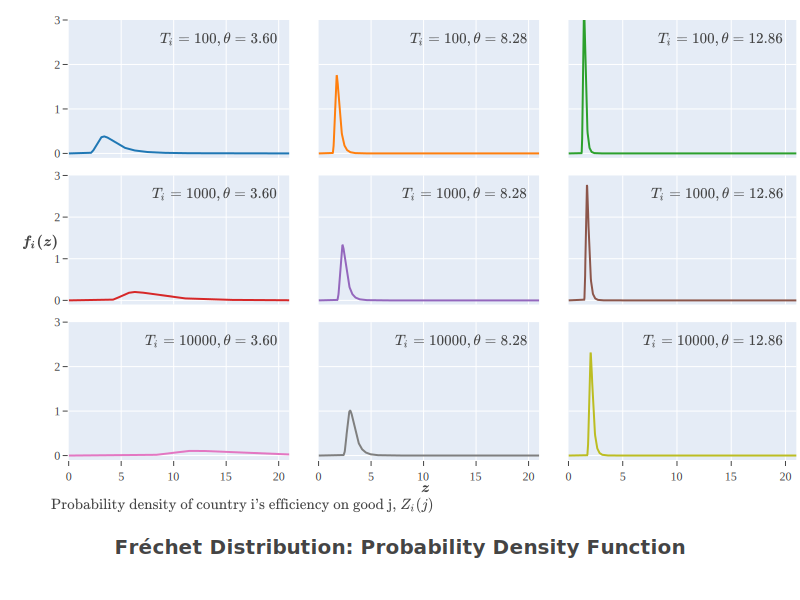
\includegraphics[width=0.9\linewidth]{./Frechet-distribution/Fréchet-distribution-density} \end{center}

如上图,为 \(Z_i\)
分布的概率密度函数,可以很直观地验证 (2)(3) 两条性质。

\hypertarget{theta-ux7684ux7ecfux6d4eux542bux4e49}{%
\subsubsection{\texorpdfstring{\(\theta\) 的经济含义}{\textbackslash theta 的经济含义}}\label{theta-ux7684ux7ecfux6d4eux542bux4e49}}

为什么说 Fréchet 分布的技术异质化程度参数 \(\theta\) 可以表征比较优势的大小?因为

\begin{enumerate}
\def\labelenumi{\arabic{enumi}.}
\tightlist
\item
  EK2002 的 (12) 式表明,\(\theta\) 越小,贸易障碍对标准化贸易份额的负面影响越小,即\textbf{贸易克服贸易障碍的能力越强}。
\item
  而在 DFS1977 中,\textbf{比较优势(两国相对生产率跨产业的异质化程度)} \(CA\) 越大,\(A(z)\) 越陡峭\footnote{在 DFS1977 框架中,我们甚至可以给出一个\textbf{比较优势的操作性定义,即} \(A(z)\) 的平均陡峭程度:\(CA_{simple} \equiv \frac{A(1)}{A(0)}\).}(注意,这个 \(z\) 是产品的编号,与 EK2002 中表示效率的 \(z\) 不同),贸易的冰山成本 \(g\) 对可贸易品范围的负面影响越小 (Section 3.B),即\textbf{贸易克服冰山成本的能力越强}。
\end{enumerate}

\begin{quote}
\[
CA(i,j) \equiv \frac{a(i)/a(j)}{a^\ast(i)/a^\ast(j)}=\frac{a(i)}{a^\ast(i)}\frac{a^\ast(j)}{a(j)}=\frac{A(j)}{A(i)}
\]
\end{quote}

\includegraphics{img/CA.png}

EK2002 与 DFS1977 相比,内在机制虽不尽相同,但这两个结论\textbf{在结构上是很相似的},因此我们可以将 \(\theta\) 称为比较优势参数\footnote{作者解释 \(\theta\) 的经济学含义时,在脚注 15 中引用了 DFS1977. 他用随机抽样方法构造了符合 Fréchet 分布的生产率数据样本,然后推导了 \(A(z)\) 与 \(T\) 的关系,表明两国的技术水平之比 \(T^\ast/T\) 越大,\(A(z)\) 越陡峭。所以除了 \(\theta\),两国技术水平之比其实也是能够表征比较优势的参数。}。

但不容易在几何上找到对 \(\theta\) 的直观解释,这与 DFS1977 不同。

\begin{quote}
从几何直观来看,\(\theta\) 意味着一国产业效率的异质化程度。

\(\theta \rightarrow \infty\) 时,Fréchet 分布的概率密度函数在 \(z=1\) 处塌缩为一个高度为无穷大的尖峰,意味着一国所有产业的效率相同,价格也相同。用 DFS1977 的观点看,则 \(\begin{aligned} \frac{A(j)}{A(i)}=\frac{a(i)/a(j)}{a^\ast(i)/a^\ast(j)}=\frac{1}{1}=1 \end{aligned}\),\(A(z)\) 曲线是平的,若有贸易障碍,会吞噬所有的可贸易品范围。

\(\theta \rightarrow 0\) 时,Fréchet 分布的概率密度函数是一条高度非常低的双曲线,每个国家的生产效率都有广泛的分布。在大数定律下,对于任一产品门类,两国的生产效率之比 \(a^\ast(j)/a(j)=A(j)\) 可以从接近零变异到无穷大。用 DFS1977 的观点看, \(A(z)\) 的变化从最低的接近零变化到最高的趋于无穷大,非常陡峭,则贸易克服贸易障碍的能力会非常强。
\end{quote}

\hypertarget{ux4ef7ux683c}{%
\subsection{价格}\label{ux4ef7ux683c}}

\hypertarget{ux4ef7ux683cux5206ux5e03}{%
\subsubsection{价格分布}\label{ux4ef7ux683cux5206ux5e03}}

首先求 \(P_{ni}\) 的分布,定义其分布函数为

\[
G_{ni}(p) \equiv Pr[P_{ni} \le p]  
\]

则有:

\[
G_{ni}(p) =1-e^{-T_{i} ( {{c_i}d_{ni}})^{-\theta}p^{\theta}} \tag{5}
\]

\begin{quote}
证明 (5) 式:
\[
\begin{aligned}
G_{ni}(p) & \equiv Pr[P_{ni} \le p] \\  
&= Pr[\frac {{c_i}d_{ni}}{Z_i} \le p]  = Pr[Z_i \geq \frac {{c_i}d_{ni}}{p}] \\ & = 1-Pr[Z_i \le \frac {{c_i}d_{ni}}{p}] = 1 - F_i(\frac {{c_i}d_{ni}}{p}) \\  
&= 1 - e^{-T_{i} (\frac {{c_i}d_{ni}}{p})^{-\theta}} = 1-e^{-T_{i} ( {{c_i}d_{ni}})^{-\theta}p^{\theta}} \quad \blacksquare 
\end{aligned}
\]
\end{quote}

这是 \(i\) 国出口到 \(n\) 国的某种产品价格小于等于 \(p\) 的概率,经过市场竞争,最终
\(n\) 国该种产品的价格小于等于 \(p\) 的概率为

\[
G_n(p) =1-\prod_{i}{(1-G_{ni}\left(p\right))}
\]

\begin{quote}
证明:\[\begin{aligned}
G_n(p) &= Pr[P_n \le p] \\ 
&=Pr[ \min \left\{P_{n i} ; i=1, \cdots, N\right\} \le p] \\ 
&= 1 - Pr[ \min \left\{P_{n i} ; i=1, \cdots, N\right\} \geq p] \\ 
&= 1- Pr[ P_{n i}  \geq p; i=1, \cdots, N]\\ &=1-\prod_{i}Pr\left\{P_{ni}\geq p\right\} \\ 
&=1-\prod_{i}{(1-G_{ni}\left(p\right))} \quad \blacksquare 
\end{aligned}\]
\end{quote}

将 (5) 式代入,得

\[
G_n\left(p\right)=1-e^{-[\sum_{i=1}^{N}T_{i} ( {{c_i}d_{ni}})^{-\theta}]p^{\theta}} 
\]

将其记为

\[
G_{n}(p)=1-e^{-\Phi_{n} p^{\theta}}  \tag{6}
\]

其中,定义价格参数

\[
\Phi_{n} = \sum_{i=1}^{N}T_{i} ( {{c_i}d_{ni}})^{-\theta} \tag{7}
\]

价格参数 \(\Phi_n\) 非常重要,因为它包含了影响各国价格的3个因素:(1)技术水平
\(T_i\);(2)要素成本 \(c_i\);(3)地理障碍 \(d_{ni}\)。

\hypertarget{phi_n-ux7684ux6027ux8d28}{%
\subsubsection{\texorpdfstring{\(\Phi_n\) 的性质}{\textbackslash Phi\_n 的性质}}\label{phi_n-ux7684ux6027ux8d28}}

\begin{enumerate}
\def\labelenumi{\arabic{enumi}.}
\tightlist
\item
  国家数量越多,或国家数量不变而 \(T_i\) 越大,都会使 \(\Phi_n\) 越大,从而
  \(G_{n}(p)\)
  越大,即价格的期望会越小。因此,\textbf{更广泛的国际贸易}可以使本国居民享受到更低的价格水平,\textbf{就像各国技术提高了一样}。
\item
  国际贸易的利得会受到要素成本和地理障碍的削弱。考虑两种极端情况:

  \begin{enumerate}
  \def\labelenumii{\alph{enumii}.}
  \tightlist
  \item
    零障碍,即 \(d_{n i} \equiv 1, \forall n, i\),此时
    \(\Phi_{n} = \sum_{i=1}^{N}T_{i}{c_i}^{-\theta}\)
    对于所有国家都一样,从而各国价格的分布函数一致。这就是概率版本的一价定律:各国价格的概率分布完全相同(但具体到某种产品,实际价格通常不同)
  \item
    自给自足,即 \(d_{n i} \rightarrow \infty, \forall n \neq i\),此时
    \(\Phi_{n} = T_{n}{c_n}^{-\theta}\),价格只受本国技术和要素成本影响。
  \end{enumerate}
\end{enumerate}

\hypertarget{ux4ef7ux683cux5206ux5e03ux7684ux4e09ux4e2aux6027ux8d28}{%
\subsubsection{价格分布的三个性质}\label{ux4ef7ux683cux5206ux5e03ux7684ux4e09ux4e2aux6027ux8d28}}

\hypertarget{ux6027ux8d281}{%
\paragraph{性质1}\label{ux6027ux8d281}}

\(n\) 国最终选择从 \(i\) 国购买某种产品 \(j\) 的概率为

\[
\pi_{n i}=\frac{T_{i}\left(c_{i} d_{n i}\right)^{-\theta}}{\Phi_{n}} \tag{8}
\]

\begin{quote}
证明 (8) 式: 由于独立同分布,\(N\) 维空间中的联合概率密度函数可以表示为
\(N\) 个概率密度函数的积\[\begin{aligned}
\pi_{n i}&=\operatorname{Pr}\left[P_{n i} \leq \min \left\{P_{n s}; s \neq i\right\}\right] \\ 
&=\int\cdots\int_{\left[P_{n i} \leq \min \left\{P_{n s}; s \neq i\right\}\right]}{ f(p_{n 1}, \cdots ,p_{n n}) d p_{n 1} \cdots d p_{n n}}\\
&=\int\cdots\int_{\left[P_{n i} \leq \min \left\{P_{n s}; s \neq i\right\}\right]}{ \prod_{i=1}^{N}f_{ni}(p_{ni})d p_{n 1} \cdots d p_{n n}}\\
&={\int_{0}^{\infty} f_{n i}(p_{ni})\left[\prod_{s \neq i} \int_{p_{ni}}^{\infty}f_{n s}(p_{ns}) d p_{n s}\right] d p_{ni}}\\
&={\int_{0}^{\infty} f_{n i}(p_{ni})\prod_{s \neq i} \left [1 - G_{n s}(p_{ni})\right] dp_{ni}} \\
&=\int_{0}^{\infty} \prod_{s \neq i}\left[1-G_{n s}(p_{ni})\right] d G_{ni}(p_{ni}) \\ 
&=\int_{0}^{\infty} \prod_{s \neq i}e^{ -T_{s}\left(c_{s} d_{n s}\right)^{-\theta} p_{ni}^{\theta}} \cdot e^{ -T_{i}\left(c_{i} d_{n i}\right)^{-\theta} p_{ni}^{\theta}} T_{i}\left(c_{i} d_{n i}\right)^{-\theta} d p_{ni}^{\theta}\\
&=T_{i}\left(c_{i} d_{n i}\right)^{-\theta}\int_{0}^{\infty} e^{ -\Phi_n p_{ni}^{\theta}}  d p_{ni}^{\theta}\\
&=\frac{T_{i}\left(c_{i} d_{n i}\right)^{-\theta}}{\Phi_{n}} \quad \blacksquare \end{aligned}\]
\end{quote}

同时,\(\pi_{ni}\) 也是 \(\Phi_{n}\) 中 \(i\) 国的贡献比例。

由无限种商品连续统的假设,结合大数定律知,\(n\) 国最终从 \(i\) 国购买的产品种类占
\(n\) 国消费全部产品种类的比例也是 \(\pi_{ni}\).

\hypertarget{ux6027ux8d282}{%
\paragraph{性质2}\label{ux6027ux8d282}}

\(n\) 国最终选择从 \(i\) 国购买某种产品,其价格的条件概率分布也是 \(G_{n}(p)\)。

\begin{quote}
证明该条件概率分布:\[
\begin{aligned}
& \operatorname{Pr}\left[ P_{n i} \leq p \mid P_{n i} \leq \min \left\{P_{n s}; s \neq i\right\}\right] \\ 
=& \frac{\operatorname{Pr}\left[P_{n i} \leq p, P_{n i} \leq \min \left\{P_{n s}; s \neq i\right\}\right]}{\operatorname{Pr}\left[P_{n i} \leq \min \left\{P_{n s}; s \neq i\right\}\right]}\\ 
=& \frac{\int \cdots \int_{\left[P_{n i} \leq p, P_{n i} \leq \min \left\{P_{n s}; s \neq i\right\}\right]} \prod_{i = 1}^{N} f_{n i}\left(p_{n i}\right) d p_{n 1} \ldots d p_{n n}}{\pi_{n i}}\\ 
=& \frac{\int_{0}^{p} f_{n i}\left(p_{n i}\right)\left[\prod_{s \neq i} \int_{p_{n i}}^{\infty} f_{n s}\left(p_{n s}\right) d p_{n s}\right] d p_{n i}}{\pi_{n i}}\\ 
=& \frac{\int_{0}^{p} f_{n i}\left(p_{n i}\right) \prod_{s \neq i}\left[1-G_{n s}\left(p_{n i}\right)\right] d p_{n i}}{\pi_{n i}}\\ 
=& \frac{\int_{0}^{p} \prod_{s \neq i}\left[1-G_{n s}\left(p_{n i}\right)\right] d G_{n i}\left(p_{n i}\right)}{\pi_{n i}}\\
=& \frac{\left[T_{i}\left(c_{i} d_{n i}\right)^{-\theta}\right]\int_{0}^{p} e^{-\Phi_{n} p_{n i}^{\theta}} d p_{n i}^{\theta}}{\pi_{n i}}\\ 
=& 1-e^{-\Phi_{n} p^{\theta}} \\
=& G_n(p) \quad \blacksquare 
\end{aligned}\]
\end{quote}

由大数定律知,最终 \(n\) 国从 \(i\) 国进口的所有产品的价格分布也是
\(G_{n}(p)\)。因此,不同来源国产品价格的概率分布一致。

如何理解这条性质呢?由 (11) 式知,技术水平高、投入成本低、到 \(n\)
国地理障碍少的国家,以所有产品计算,到达 \(n\)
国的商品到岸价格的均值会更低。但事实上,\(n\)
国只会购买该国生产最有效率的一部分产品。而对于缺乏竞争优势的国家,虽然以所有产品计算,到达
\(n\) 国的商品到岸价格的均值会高一些,但 \(n\)
国购买其产品更少,集中在其最有竞争力的商品上。最终,A source with a higher state
of technology, lower input cost, or lower barriers exploits its advantage by
selling a wider range of goods, exactly to the point at which the distribution
of prices for what it sells in \(n\) is the same as \(n\)'s overall price
distribution. 两国在 \(n\) 国出售商品的价格分布刚好一致。

比如,德国技术水平高,在许多产品中具有价格优势;西班牙技术水平低,具有价格优势的产品品种就比较少。但是,如果本国购买更多种类的德国产品,而只买很少数量的西班牙最有竞争力的产品,则最终对两国产品的平均购买价格可能是一样的。

\hypertarget{ux6027ux8d283}{%
\paragraph{性质3}\label{ux6027ux8d283}}

在 \(\sigma < 1 + \theta\) 的前提下\footnote{\(\Gamma\) 分布要求参数 \(\frac{1+\theta-\sigma}{\theta}>0\),所以必须有
  \(\sigma < 1 + \theta\).},CES 效用函数对应的价格指数\footnote{第四部分中可以推导,对于 CES 效用函数,有价格指数
  \(p=\left[\int_0^1 p(j)^{1-\sigma}dj\right]^{\frac{1}{1-\sigma}}\),满足
  \(U=I/p\)。因此,求出该价格指数对于计算效用是非常方便的。}

\[
p_{n}=\gamma \Phi_{n}^{-1 / \theta}  \tag{9}
\]

其中
\(\gamma=\left[\Gamma\left(\frac{\theta+1-\sigma}{\theta}\right)\right]^{1 /(1-\sigma)}\).

因各国的 \(\Phi_{n}\)
受到地理障碍的影响而不同,故各国的价格指数不同。因此,地理障碍这个因素使各国价格偏离一价定律,且越远离其他国家的国家,其价格指数越大。

\begin{quote}
证明: \(n\) 国价格指数为
\(p_n=\left[\int_0^1 p_n(j)^{1-\sigma}dj\right]^{\frac{1}{1-\sigma}}\).
方括号中的统计量实际上是对商品连续统的一个积分,可以将其写成面积和的形式:将
\([0,1]\) 区间划分为 \(S\)
份,计算每份的面积:\(\int_0^1 p_n(j)^{1-\sigma}dj=\lim_{S \to \infty} \sum_{k=1}^{S} \left[\frac{1}{S}\cdot p_{n}(k)^{1-\sigma}\right]\)
由于 \(p_n(k)\sim G_n(p)\) 独立同分布,上式中的面积和可以视为同一个随机变量
\((P_n)^{1-\sigma}\) 多次抽样的均值
\(\frac{1}{S}\cdot\sum_{k=1}^{S} p_{n}(k)^{1-\sigma}\)。当抽样次数趋于无穷大时,根据大数定律,该均值等于
\((P_n)^{1-\sigma}\) 的期望。则 \[\begin{aligned}
\int_0^1 p_n(j)^{1-\sigma}dj & = E\left[P_n^{1-\sigma}\right] = \int_{0}^{\infty}p^{1-\sigma}f_n(p)dp \\
&= \int_{0}^{\infty}p^{1-\sigma}dG_n(p)=\int_{0}^{\infty }p^{1-\sigma}e^{-\Phi_n p^\theta} d(\Phi_n p^\theta) \\
& \stackrel{\text{令 }x=\Phi_n p^{\theta}}{=} \int_{0}^{\infty}\left(x/\Phi_n\right)^{\frac{1-\sigma}{\theta}}e^{-x}dx \\
&= \Phi_n^{-\frac{1-\sigma}{\theta}}\int_{0}^{\infty }x^{\frac{1+\theta-\sigma}{\theta}-1}e^{-x}dx \\
&=\Phi_n^{-\frac{1-\sigma}{\theta}}\Gamma (\frac{1+\theta-\sigma}{\theta})
\end{aligned}\] 从而
\[ p_n=\Phi_n^{-\frac{1}{\theta}}\left[\Gamma (\frac{1+\theta-\sigma}{\theta})\right]^{\frac{1}{1-\sigma}}=\gamma \Phi_n^{-\frac{1}{\theta}} \quad \blacksquare \]
\end{quote}

\hypertarget{ux8d38ux6613ux6d41ux91cfux548cux5f15ux529b}{%
\subsection{贸易流量和引力}\label{ux8d38ux6613ux6d41ux91cfux548cux5f15ux529b}}

由上一节价格分布的性质 2 知,\(n\) 国消费的每种产品的价格分布与来源地无关,均服从
\(G_n(p)\)。在连续统商品的假设下,\(n\) 国从每个国家都购买了无穷多种商品,则 \(n\)
国从每个国家购买的商品的平均价格都应严格等于 \(G_n(p)\)
这个分布所对应的期望,是相同的。因此 \(n\)
国从一个国家的进口支出与从该国进口的商品数量成正比。

又因为效用函数是对称的,在所有商品价格服从同一分布的前提下,其消费数量也服从同一分布。故由大数定律,从一国进口商品的数量与进口商品的种类成正比。因此,\(n\)
国从 \(i\) 国进口支出占 \(n\) 国制造业总支出的比例,就等于 \(n\) 国从 \(i\)
国进口商品种类占所有消费商品种类的比例,由性质 1 知,该比例为 \(\pi_{ni}\),即:

\[
\frac{X_{n i}}{X_{n}}=\pi_{ni}=\frac{T_{i}\left(c_{i} d_{n i}\right)^{-\theta}}{\Phi_{n}}=\frac{T_{i}\left(c_{i} d_{n i}\right)^{-\theta}}{\sum_{k=1}^{N} T_{k}\left(c_{k} d_{n k}\right)^{-\theta}}  \tag{10}
\]

其中,\(X_{n}\) 为 \(n\) 国制造业总支出,\(X_{n i}\) 为 \(n\) 国自 \(i\) 国的制造业产品进口额。

\(i\) 国制造业的总收入为:

\[
Q_{i}=\sum_{m=1}^{N} X_{m i}=T_{i} c_{i}^{-\theta} \sum_{m=1}^{N} \frac{d_{m i}^{-\theta} X_{m}}{\Phi_{m}}
\]

由此可得

\[
T_{i} c_{i}^{-\theta}=Q_i/\sum_{m=1}^{N} \frac{d_{m i}^{-\theta} X_{m}}{\Phi_{m}}
\]

将其代入 (10) 式并结合 (9) 式得到

\[
X_{n i}=\frac{\left(\frac{d_{n i}}{p_{n}}\right)^{-\theta} X_{n}}{\sum_{m=1}^{N}\left(\frac{d_{m i}}{p_{m}}\right)^{-\theta} X_{m}} Q_{i} \tag{11}
\]

\begin{enumerate}
\def\labelenumi{(\arabic{enumi})}
\setcounter{enumi}{10}
\tightlist
\item
  式是一个标准的\textbf{引力方程}。它具有以下性质:(1)双边贸易额对 \(n\) 国制造业产品总支出 \(X_n\) 和 \(i\) 国制造业总收入 \(Q_i\) 的弹性为1\footnote{前提是 \(N\) 充分大,或 \(n\) 国为一个小国。}。(2)地理障碍 \(d_{ni}\) 被进口国的价格指数 \(p_n\)
  缩减。给定 \(i\) 国的总出口额 \(Q_i\),可以将 (11) 式右边的分母视为 \(i\) 国眼中的全球市场,则分子与分母的比就是 \(n\) 国所占份额。\(p_n\)
  的下降与地理障碍 \(d_{ni}\) 的上升具有相同的作用,即阻碍 \(i\) 国产品进入 \(n\)
  国(地理障碍越大,进口国本国物价越便宜,出口国的商品越不容易进来)。
\end{enumerate}

\hypertarget{estimate-partial-equilibrium}{%
\section{贸易、地理和价格初探}\label{estimate-partial-equilibrium}}

\hypertarget{ux6807ux51c6ux5316ux7684ux8fdbux53e3ux4efdux989d}{%
\subsection{标准化的进口份额}\label{ux6807ux51c6ux5316ux7684ux8fdbux53e3ux4efdux989d}}

在 (10) 式中取 \(n\) 为 \(i\),然后再相除,得到

\[
\frac{X_{n i} / X_{n}}{X_{i i} / X_{i}}=\frac{\Phi_{i}}{\Phi_{n}} d_{n i}^{-\theta}=\left(\frac{p_{i} d_{n i}}{p_{n}}\right)^{-\theta} \tag{12}
\]

\begin{enumerate}
\def\labelenumi{(\arabic{enumi})}
\setcounter{enumi}{11}
\tightlist
\item
  式左边为 \(i\) 国产品在 \(n\) 国制造业产品支出中的占比除以 \(i\) 国产品在 \(i\)
  国造业产品支出中的占比,称为标准化的 \(n\) 国进口中来源于 \(i\) 国的份额(\(n\)'s normalized
  import share from \(i\),简称为标准化贸易份额)。
\end{enumerate}

\begin{itemize}
\tightlist
\item
  标准化贸易份额不会超过1。因为,\(\frac{X_{n i} / X_{n}}{X_{i i} / X_{i}}>1 \Rightarrow \frac{p_{i} d_{n i}}{p_{n}}<1\),若该式成立,\(n\)
  国消费的所有产品都可以从 \(i\) 国进口以节省开支(a purchaser in country \(n\)
  can always buy all her goods in \(i\) at a price index \(p_{i} d_{n i}\)),这与
  \(n\) 国选择了最低价格是矛盾的
\item
  性质

  \begin{itemize}
  \tightlist
  \item
    \(p_i/p_n\)↗ 或 \(d_{ni}\)↗ 使标准化贸易份额下降
  \item
    \(\theta\)↗ 反映比较优势减弱,可贸易范围减少,使标准化贸易份额下降
  \end{itemize}
\end{itemize}

\hypertarget{trade-price-estimate}{%
\subsection{\texorpdfstring{估计 \(\theta\)}{估计 \textbackslash theta}}\label{trade-price-estimate}}

第 (12) 式两边取对数后,\(\theta\) 成为斜率。因此可以用这个方程估计 \(\theta\).

\hypertarget{ux8ba1ux7b97ux6807ux51c6ux5316ux8fdbux53e3ux4efdux989d}{%
\subsubsection{计算标准化进口份额}\label{ux8ba1ux7b97ux6807ux51c6ux5316ux8fdbux53e3ux4efdux989d}}

可以使用制造业进出口数据计算标准化贸易份额。

在无贸易障碍的世界,\(d_{ni}=1, \forall n, i\),所有的 \(\Phi\)
都相等,从而所有的价格水平 \(p\) 都相等,则由 (12) 式知标准化的贸易份额将等于 1. 但现实数据显示,该份额从未超过
0.2,且在不同国家对之间差别很大------超过 4 个数量级,如 Figure 1 所示:

\begin{center}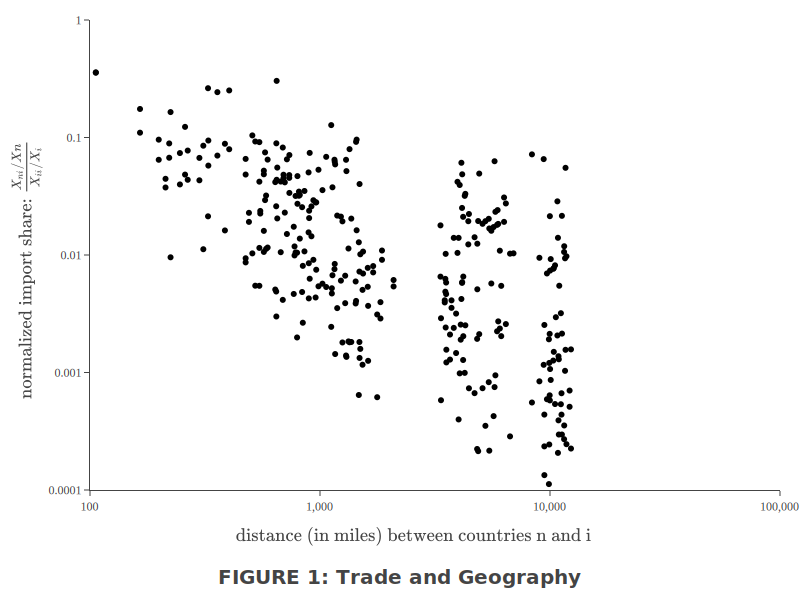
\includegraphics[width=0.9\linewidth]{img/Figure1} \end{center}

这说明,地理(障碍)因素对贸易的影响相当显著。

\hypertarget{ux8ba1ux7b97-price-measure}{%
\subsubsection{计算 price measure}\label{ux8ba1ux7b97-price-measure}}

价格指数之比:取 50 种产品在样本国家中的零售数据,并进行对数化处理:\(r_{n i}(j) \equiv \ln p_{n}(j)-\ln p_{i}(j)\)。对这 50 种产品的 \(-r_{n i}(j)\) 取平均值,作为 \(\ln \frac{p_i}{p_n}\) 的代理变量(proxy)

\(d_{ni}\) 不是简单的运输成本,而是对所有贸易障碍的衡量,无法直接计算,只能找代理变量。按照本文的理论,只有 \(n\) 国从 \(i\) 国进口的产品才满足 \(p_n(j)/p_i(j)=d_{ni} \Rightarrow r_{ni}(j)=\ln d_{ni}\),\(n\) 国从第三国进口的产品 \(k\) 的价格比从 \(i\) 国进口更便宜,因此有 \(p_n(k)<p_i(k)\cdot d_{ni} \Rightarrow r_{ni}(k)<\ln d_{ni}\)。即 \(\ln d_{ni}\) 是 \(r_{ni}(j)\) 的上限,故有 \(\max\left\{ r_{ni}(j); j \in [0,1]\right\}=\ln d_{ni}\). 因此,用第二大的 \(r_{n i}(j)\) 作为 \(\ln d_{ni}\) 的代理变量(不选第一大是为了避免异常值的影响)。

以

\[
D_{n i} \equiv \max 2_{j}\left\{r_{n i}(j)\right\}-\frac{1}{50}\sum_{j=1}^{50}\left[r_{n i}(j)\right] \tag{13}
\]

作为 \(\ln ({p_{i} d_{n i}}/{p_{n}})\) 的代理变量\footnote{\(\max 2\{\}\)\hspace{0pt} 表示第二大。原文中此式有误,勘误表中已经指出,见 \href{https://drive.google.com/viewerng/viewer?a=v\&pid=sites\&srcid=eWFsZS5lZHV8a29ydHVtfGd4OjU1YzE1YTIxYTJlNzA3MjE}{TGT
  Corrections.pdf
  (google.com)}.}。

将 \(exp(D_{n i})\) 命名为 price measure,表示一个 \(n\) 国人若全部从 \(i\)
国购买商品,比实际的购买(充分按照比较优势)会贵多少(a buyer who insisted on
purchasing everything from source \(i\), relative to the actual price index in
\(n\), the price index for a buyer purchasing each goodfrom the cheapest
source)。

\begin{center}\includegraphics[width=0.9\linewidth]{img/Table2} \end{center}

一些计算出的 price measure 值,整理在 Table 2 中。

图中法国那一行显示,法国最便宜的货源在德国(第 1
列),从德国购买所有商品只需多支付 33\%;最昂贵的货源是新西兰(第 2
列),从新西兰购买所有商品要多支付
142\%。一个坚持从法国购买所有商品的海外居民,如果在比利时(第 3
列),将面临最小的惩罚(40\%);如果在日本(第 4 列),将面临最大的惩罚(140\%)。

最便宜的外国货源通常在附近,而最贵的则在远处。从第 4
列来看,如果要求必须从某个外国来源购买所有的东西,大国通常会受到最大的不利影响(美国、日本出现最频繁)。

\hypertarget{ux53c2ux6570ux4f30ux8ba1}{%
\subsubsection{参数估计}\label{ux53c2ux6570ux4f30ux8ba1}}

有了标准化进口份额和 \(D_{n i}\),便可以利用 (12) 式估计 \(\theta\),如
Figure 2 所示:

\begin{center}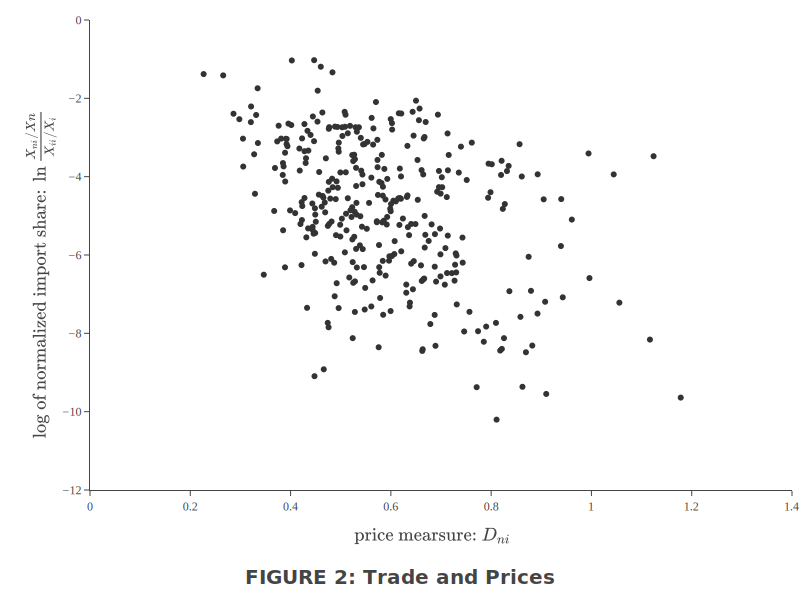
\includegraphics[width=0.9\linewidth]{img/Figure2} \end{center}

由于 (12) 式的结构意味着截距为 0,因此可以使用最简单的一阶矩估计:标准化贸易份额的对数取平均值除以 \(D_{ni}\)
的平均值,估计的 \(\theta\) 为 8.28(其他的估计方法得到的 \(\theta\)
值在同一个数量级范围内),这个大小意味着效率分布的标准差为均值的大约 \(17.2\%\).

\begin{Shaded}
\begin{Highlighting}[]
\NormalTok{theta }\OtherTok{\textless{}{-}} \FloatTok{8.28}

\CommentTok{\# 一系列不同的 T}
\NormalTok{T\_list }\OtherTok{\textless{}{-}} \FunctionTok{seq}\NormalTok{(}\DecValTok{1}\NormalTok{, }\DecValTok{4}\NormalTok{, }\AttributeTok{length.out =} \DecValTok{10}\NormalTok{) }\SpecialCharTok{\%\textgreater{}\%}
  \StringTok{\textasciigrave{}}\AttributeTok{*}\StringTok{\textasciigrave{}}\NormalTok{(}\FunctionTok{log}\NormalTok{(}\DecValTok{10}\NormalTok{)) }\SpecialCharTok{\%\textgreater{}\%}
  \FunctionTok{exp}\NormalTok{()}

\NormalTok{T\_list }\SpecialCharTok{\%\textgreater{}\%} \FunctionTok{map\_dbl}\NormalTok{(}\ControlFlowTok{function}\NormalTok{(T) \{}
  \CommentTok{\# 概率密度}
\NormalTok{  f }\OtherTok{\textless{}{-}} \ControlFlowTok{function}\NormalTok{(x) \{}
\NormalTok{    T }\SpecialCharTok{*}\NormalTok{ theta }\SpecialCharTok{*}\NormalTok{ x}\SpecialCharTok{\^{}}\NormalTok{(}\SpecialCharTok{{-}}\NormalTok{theta }\SpecialCharTok{{-}} \DecValTok{1}\NormalTok{) }\SpecialCharTok{*} \FunctionTok{exp}\NormalTok{(}\SpecialCharTok{{-}}\NormalTok{T }\SpecialCharTok{*}\NormalTok{ (x}\SpecialCharTok{\^{}}\NormalTok{(}\SpecialCharTok{{-}}\NormalTok{theta)))}
\NormalTok{  \}}

  \CommentTok{\# 期望}
\NormalTok{  E }\OtherTok{\textless{}{-}} \FunctionTok{integrate}\NormalTok{(}\ControlFlowTok{function}\NormalTok{(x) \{}
\NormalTok{    x }\SpecialCharTok{*} \FunctionTok{f}\NormalTok{(x)}
\NormalTok{  \}, }\DecValTok{0}\NormalTok{, }\DecValTok{25}\NormalTok{)}\SpecialCharTok{$}\NormalTok{value }\CommentTok{\# 积分限制在(0, 25)这个区间,精度足够}

  \CommentTok{\# 标准差}
\NormalTok{  sigma }\OtherTok{\textless{}{-}} \FunctionTok{integrate}\NormalTok{(}\ControlFlowTok{function}\NormalTok{(x) \{}
\NormalTok{    (x }\SpecialCharTok{{-}}\NormalTok{ E)}\SpecialCharTok{\^{}}\DecValTok{2} \SpecialCharTok{*} \FunctionTok{f}\NormalTok{(x)}
\NormalTok{  \}, }\DecValTok{0}\NormalTok{, }\DecValTok{25}\NormalTok{)}\SpecialCharTok{$}\NormalTok{value }\SpecialCharTok{\%\textgreater{}\%} \FunctionTok{sqrt}\NormalTok{()}

  \CommentTok{\# 返回一系列 T 对应的 sigma/E}
\NormalTok{  sigma }\SpecialCharTok{/}\NormalTok{ E}
\NormalTok{\})}
\end{Highlighting}
\end{Shaded}

\begin{verbatim}
#>  [1] 0.1722408 0.1722408 0.1722407 0.1722407 0.1722406 0.1722403 0.1722400
#>  [8] 0.1722393 0.1722382 0.1722363
\end{verbatim}

\hypertarget{ux5b8cux5907ux6a21ux578b14}{%
\section[完备模型]{\texorpdfstring{完备模型\footnote{将要素价格作为内生变量,求一般均衡。}}{完备模型}}\label{ux5b8cux5907ux6a21ux578b14}}

前面讨论的(1)双边贸易流(2)价格和地理的关系都建立在要素价格外生的前提下。本节将要素价格内生化。

\ref{input-price}
节在劳动力价格给定条件下讨论中间产品价格的决定,\ref{factor-price}
节对劳动力价格建立一般均衡模型。

\hypertarget{ux751fux4ea7}{%
\subsection{生产}\label{ux751fux4ea7}}

\hypertarget{ux751fux4ea7ux51fdux6570ux4e0eux4e24ux9636ux6bb5ux6700ux4f18ux5316}{%
\subsubsection{生产函数与两阶段最优化}\label{ux751fux4ea7ux51fdux6570ux4e0eux4e24ux9636ux6bb5ux6700ux4f18ux5316}}

假设生产要使用劳动和中间投入品,且生产函数为适用两阶段最优化的 D-S Lite 型,见
\citet{DS1977} ,即:(1)总成本中劳动 \(L\) 所占份额 \(\beta\) 保持不变;(2)中间品投入
\(Q(j)\) 以 CES 方式组织起来。具体形式如下(各国生产函数只有表示效率的 \(z_i(j)\)
这个唯一的区别):

\[
y_{i}(j)=\frac{z_{i}(j)}{\beta^{\beta}(1-\beta)^{1-\beta}} L^{\beta}\left\{\left[\int_{0}^{1} Q(j)^{\frac{\sigma-1}{\sigma}} d j\right]^{\frac{\sigma}{\sigma-1}}\right\}^{1-\beta}
\]

则成本最小化问题为

\[
\left\{\begin{array}{c}
{\min_{L, Q} w_{i}L + \int_{0}^{1} P_{i}(j)Q(j) d j} \\ {\text { s.t. }\frac{z_{i}(j)}{\beta^{\beta}(1-\beta)^{1-\beta}} L^{\beta}\left\{\left[\int_{0}^{1} Q(j)^{\frac{\sigma-1}{\sigma}} d j\right]^{\frac{\sigma}{\sigma-1}}\right\}^{1-\beta}=y_{i}(j)}
\end{array}\right.
\]

为便于求解,将其对偶化为产量最大化问题,并进行三个换元

\begin{itemize}
\tightlist
\item
  令效率指数 \(k_{i}(j)=\frac{z_{i}(j)}{\beta^{\beta}(1-\beta)^{1-\beta}}\)
\item
  令中间品数量指数
  \(K=\left[\int_{0}^{1} Q(j)^{\frac{\sigma-1}{\sigma}} d j\right]^{\frac{\sigma}{\sigma-1}}\)
\item
  令中间品价格指数
  \(p_{i}(j)=\left[\int_{0}^{1} P_{i}(j)^{1-\sigma} d j\right]^{\frac{1}{1-\sigma}}\),可以证明其为
  \(\gamma \Phi_{i}^{-1 / \theta}\),与具体产品 \(j\) 无关,故可以统一写为
  \(p_{i}\). 且有 \(p_{i}K=\int_{0}^{1} P_{i}(j)Q(j) d j\)
\end{itemize}

于是最优化问题变为

\[
\left\{\begin{array}{c}
{\max_{L, K} y_{i}(j)=k_{i}(j)L^{\beta}K^{1-\beta}} \\ {\text { s.t. } w_{i}L + p_{i}K = C}
\end{array}\right.
\]

易知均衡时 \(L^*=\beta C/w_i, K^*=(1-\beta)C/p_i\),因此 \(i\) 国生产 \(j\)
产品的单价为

\[\frac{C}{y_{i}(j)}=\frac{C}{k_i(j)\left(\frac{\beta C}{w_i}\right)^\beta\left[\frac{(1-\beta) C}{p_i}\right]^{1-\beta}}=\frac{w_{i}^{\beta}p_{i}^{1-\beta}}{z_{i}(j)}\]

而由 (1) 式知该价格为 \(c(i)/{z_{i}(j)}\),故有

\[
c(i)=w_{i}^{\beta}p_{i}^{1-\beta} \tag{14}
\]

\hypertarget{ux798fux5229ux5b9eux9645ux5de5ux8d44}{%
\subsubsection{福利(实际工资)}\label{ux798fux5229ux5b9eux9645ux5de5ux8d44}}

由 (8) 式得 \(\pi_{ii}=\frac{T_{i}c_{i}^{-\theta}}{\Phi_{i}}\),再利用 (9) 式将 \(\Phi_{i}\) 换为 \(p_{i}\),则有
\(\pi_{ii}=\frac{T_{i}p_{i}^{\theta}}{c_{i}^{\theta}\gamma^{\theta}}\),故

\[\frac{c_i}{p_i}=\frac{1}{\gamma}\left(\frac{T_i}{\pi_{ii}}\right)^{\frac{1}{\theta}}\]

结合 (14) 式可得

\[
\frac{w_i}{p_i}=\left(\frac{c_i}{p_{i}}\right)^{\frac{1}{\beta}}=\gamma^{-1/\beta}\left(\frac{T_i}{\pi_{ii}}\right)^{\frac{1}{\beta\theta}} \tag{15}
\]

由于 \(\pi_{ii}\) 是 \(i\)
国制造业产品支出中来源于本国产品的比例,显然,从自给自足到开放经济,\(\pi_{ii}\)↘,从而实际工资上升,福利改善。

\hypertarget{input-price}{%
\subsection{中间产品价格}\label{input-price}}

将 (14) 式代入 (7) 式再代入 (9) 式中得:

\[
p_{n}=\gamma\left[\sum_{i=1}^{N} T_{i}\left(d_{n i} w_{i}^{\beta} p_{i}^{1-\beta}\right)^{-\theta}\right]^{-1 / \theta} \tag{16}
\]

将工资作为外生变量,则理论上,解这个 \(N\) 元非线性方程组,就可以解出 \(p\) 向量。

把 (14) 式和 (9) 式代入 (10) 式,可得

\[
\frac{X_{n i}}{X_{n}}=\pi_{n i}=T_{i}\left(\frac{\gamma d_{n i} w_{i}^{\beta} p_{i}^{1-\beta}}{p_{n}}\right)^{-\theta} \tag{17}
\]

有 \(p\) 向量后,由 (17) 式便可求得(非标准化的)贸易份额。

\hypertarget{factor-price}{%
\subsection{要素价格}\label{factor-price}}

假设:经济中有两个部门------制造业部门和非制造业部门。后者的产品不可进行国际贸易,也不以制造业产品为中间投入\footnote{可以将该部门简单地理解为 local service 部门。}
。

\(i\) 国制造业总收入为制造业总出口加上在国内的销售,即
\(\sum_{n=1}^{N} \pi_{n i} X_{n}\),其中 \(X_n\) 为 \(n\)
国对制造业产品的总支出。则 \(i\) 国制造业部门的劳动力收入(也是 \(i\)
国制造业对劳动力的投入)为

\[
w_{i} L_{i}=\beta \sum_{n=1}^{N} \pi_{n i} X_{n} \tag{18}
\]

其中,\(L_i\) 为 \(i\) 国制造业工人数量。

另一方面,\(X_n\) 可以拆解为 \(n\) 国制造业对中间产品的支出,与 \(n\)
国所有人口对制造业最终产品支出的和。

前一项为 \((1-\beta)\sum_{k=1}^{N} \pi_{k n} X_{k}\),而由 (18) 式知
\(\sum_{k=1}^{N} \pi_{k n} X_{k}=w_nL_n/\beta\),故前一项为
\(\frac{1-\beta}{\beta} w_{n} L_{n}\).

定义 \(n\) 国对所有最终产品的支出为 \(Y_n\),其中花费在制造业产品上的占比为固定值
\(\alpha\)。则后一项为 \(\alpha Y_{n}\).

两项加总,有

\[
X_{n}=\frac{1-\beta}{\beta} w_{n} L_{n}+\alpha Y_{n} \tag{19}
\]

宏观经济学指出, \(Y_n\) 同时也是总收入,包括制造业劳动力的收入 \(Y_n^M\)
和非制造业劳动力的收入 \(Y_n^O\).

\hypertarget{ux6781ux7aefux60c5ux51b5}{%
\subsubsection{极端情况}\label{ux6781ux7aefux60c5ux51b5}}

为了便于确立一般均衡框架,考虑两种极端情境,并对非制造业作出严格的假设:

\hypertarget{ux60c5ux5883ux4e00}{%
\paragraph{情境一}\label{ux60c5ux5883ux4e00}}

劳动力可在两部门间自由流动,且各国工资 \(w_i\)
由非制造业的生产率外生给定,劳动力禀赋也是外生的,从而总收入 \(Y_n\)
是外生给定的。

结合 (18)、(19) 式可得

\[
w_{i} L_{i}=\sum_{n=1}^{N} \pi_{n i}\left[(1-\beta) w_{n} L_{n}+\alpha \beta \overline{Y_n}\right] \tag{20}
\]

将 (17) 式中的 \(\pi_{ni}\) 代入上式,得到 \(N\) 个方程,再将 (16) 式解出的 \(p_i\)
代入,可解得 \(L_{i}\) 向量。

劳动力可以跨部门流动时,技术水平会影响制造业就业规模 \(L_{i}\)。

\hypertarget{ux60c5ux5883ux4e8c}{%
\paragraph{情境二}\label{ux60c5ux5883ux4e8c}}

劳动力不能跨部门流动,各国制造业就业规模 \(L_{i}\) 外生,且非制造业收入
\(Y_n^O\) 外生(同样有非制造业的工资水平外生),则
\(Y_n=w_nL_n+\overline{Y_n^O}\). 结合 (18)、(19) 式可得

\[
w_{i} L_{i}=\sum_{n=1}^{N} \pi_{n i}\left[(1-\beta+\alpha \beta) w_{n} L_{n}+\alpha \beta \overline{Y_n^O}\right] \tag{21}
\]

将 (17) 式中的 \(\pi_{ni}\) 代入上式,得到 \(N\) 个方程,再结合 (16) 式的 \(N\) 个方程,可解出 \(p_i\) 与 \(w_{i}\) 向量。

劳动力不能跨部门流动时,技术水平会影响制造业工资和价格水平。

\hypertarget{ux96f6ux548cux65e0ux7a77ux5927ux7684ux8d38ux6613ux6210ux672c}{%
\subsection{零和无穷大的贸易成本}\label{ux96f6ux548cux65e0ux7a77ux5927ux7684ux8d38ux6613ux6210ux672c}}

\begin{quote}
\textbf{这部分在论文中的重要性很低}。
\end{quote}

按照上述两种极端情况,一般均衡模型必然有解,但很难求出解析解。

继续讨论两种特殊情况,增加一些定性认识。

\hypertarget{ux96f6ux8d38ux6613ux6210ux672c}{%
\subsubsection{零贸易成本}\label{ux96f6ux8d38ux6613ux6210ux672c}}

此时 \(d_{ni}=1\),化简 (16) 式发现 \(p_i\) 的表达式对 \(i=1,2,\cdots,N\) 是相同的,从而各国价格水平一致,一价定律成立。进一步化简 (17) 式得

\[\pi_{n i}=T_{i}\left(\frac{\gamma d_{n i} w_{i}^{\beta} p_{i}^{1-\beta}}{p_{n}}\right)^{-\theta}=T_{i}\left(\gamma w_{i}^{\beta} p_{i}^{-\beta}\right)^{-\theta}\]

从而由 (18) 式得

\[
w_{i} L_{i}=\beta \sum_{n=1}^{N} \pi_{n i} X_{n}=\beta T_{i}\left(\gamma w_{i}^{\beta} p_{i}^{-\beta}\right)^{-\theta} \sum_{n=1}^{N} X_{n}
\]

因此 \[
\frac{w_{i} L_{i}}{w_{n} L_{n}}=\frac{T_{i}\left(w_{i}^{\beta} p_{i}^{-\beta}\right)^{-\theta}}{T_{n}\left(w_{n}^{\beta} p_{n}^{-\beta}\right)^{-\theta}}=\frac{T_{i}\left(w_{i}^{\beta}\right)^{-\theta}}{T_{n}\left(w_{n}^{\beta}\right)^{-\theta}}
\]

故有 \[
\frac{w_{i}}{w_{n}}=\frac{w_i/p_i}{w_n/p_n}=\left[\frac{T_{i} / L_{i}}{T_{n} / L_{n}}\right]^{\frac{1}{1+\theta \beta}} \tag{22}
\]

和
\[\frac{L_n}{L_i}=\left(\frac{w_i}{w_n}\right)^{1+\theta\beta}\frac{T_n}{T_i}\]

讨论其含义:

\begin{enumerate}
\def\labelenumi{\arabic{enumi}.}
\tightlist
\item
  劳动力可在两部门间自由流动时,工资外生,技术水平 \(T\) 越高,制造业劳动力相对越多(越专业化于制造业)。
\item
  劳动力不能跨部门流动时,制造业劳动力数量外生,技术水平 \(T\) 越高,工资越高。
\item
  给定技术水平,一国制造业劳动力的增加将导致制造业工资的下降。
\end{enumerate}

若在零贸易成本的基础上,进一步假定经济只有制造业一个部门,则由 (16) 式得

\[
\begin{array}{l}{p_{n}=\gamma\left[\sum_{i=1}^{N} T_{i}\left(w_{i}^{\beta} p_{i}^{1-\beta} d_{n i}\right)^{-\theta}\right]^{-\frac{1}{\theta}}} \\ {\Rightarrow p=p_{i}=\gamma^{\frac{1}{\beta}}\left[\sum_{i=1}^{N} T_{i}\left(w_{i}^{\beta}\right)^{-\theta}\right]^{-\frac{1}{\theta \beta}} \quad\left(d_{n i}=1, p_{n}=p_{i}\right)}\end{array}
\]

结合 (22) 式有实际工资

\[
\begin{array}{l}{W_{i}=\frac{w_{i}}{p}=\frac{w_{i}}{\gamma^{\frac{1}{\beta}}}\left[\sum_{k=1}^{N} T_{k}\left(w_{k}^{\beta}\right)^{-\theta}\right]^{\frac{1}{\theta \beta}}} \\ {=\frac{1}{\gamma^{\frac{1}{\beta}}}\left[\sum_{k=1}^{N} T_{k}\left(\frac{w_{i}}{w_{k}}\right)^{\beta \theta}\right]^{\frac{1}{\theta \beta}}} \\ {=\frac{1}{\gamma^{\frac{1}{\beta}}}\left[\sum_{k=1}^{N} T_{k}\left(\frac{T_{i} / L_{i}}{T_{k} / L_{k}}\right)^{\frac{\beta \theta}{1+\theta \beta}}\right]^{\frac{1}{\theta \beta}}}\end{array}
\]

因此

\[
W_{i}=\gamma^{-\frac{1}{\beta}} T_{i}^{\frac{1}{1+\theta \beta}}\left[\sum_{k=1}^{N} T_{k}^{\frac{1}{1+\theta \beta}}\left(L_{k} / L_{i}\right)^{\frac{\beta \theta}{1+\theta \beta}}\right]^{\frac{1}{\theta \beta}} \tag{23}
\]

可见,任何国家的技术水平 \(T_k\) 提高,\(i\) 国的福利都会上升。

\(i\) 国自身技术水平提高时,会带来额外收益,因为它将提高本国对外国的相对工资。

\(i\) 国从 \(k\) 国技术水平 \(T_k\) 的提高中获得的收益大小取决于 \(k\) 国相对于 \(i\)
国的劳动力数量。如果技术进步来源国 \(k\) 国的劳动力数量比较少,\(w_k\)
上升得更多,减少了 \(k\) 国技术水平提高给其他国家带来的利得。

\hypertarget{ux65e0ux7a77ux5927ux8d38ux6613ux6210ux672c}{%
\subsubsection{无穷大贸易成本}\label{ux65e0ux7a77ux5927ux8d38ux6613ux6210ux672c}}

此时 \(d_{n i} \rightarrow \infty, \forall n \neq i\). 在 (15) 式中取
\(\pi_{ii}=1\),得

\[
\quad W_{i}=\gamma^{-1 / \beta} T_{i}^{1 / \theta \beta}=\gamma^{-\frac{1}{\beta}} T_{i}^{\frac{1}{1+\theta \beta}}\left(T_{i}^{\frac{1}{1+\theta \beta}}\right)^{\frac{1}{\theta \beta}} \tag{24}
\]

比较发现,(23) 式的右边比 (24) 式大(后者只是前者连加式中的一项),因此每个国家均从贸易中受益了。

\hypertarget{estimate-general-equilibrium}{%
\section{估计贸易方程}\label{estimate-general-equilibrium}}

四个方程 (16)、(17)、(20)、(21) 构成了一个一般均衡模型,决定了价格水平、贸易份额、制造业工资(劳动力不可跨部门流动)或者制造业就业(劳动力可以跨部门流动)。这一部分我们主要估计一般均衡模型的诸参数,然后在 Section 6 进行反事实分析。

\hypertarget{ux4f30ux8ba1ux865aux62dfux53d8ux91cf}{%
\subsection{估计虚拟变量}\label{ux4f30ux8ba1ux865aux62dfux53d8ux91cf}}

第 (17) 式将双边贸易量同两国各自的特征以及地理信息联系了起来,对该式的估计使我们可以了解技术水平与地理障碍。

使用进口国的国内开支对 (17) 式的双边贸易数据进行标准化,令
\(\frac{X_{ni}}{X_n}\) 与 \(\frac{X_{nn}}{X_n}\) 相除可得

\[
\frac{X_{n i}}{X_{n n}}=\frac{\pi_{n i}}{\pi_{n n}}=\frac{T_{i}}{T_{n}}\left(\frac{w_{i}}{w_{n}}\right)^{-\theta \beta}\left(\frac{p_{i}}{p_{n}}\right)^{-\theta(1-\beta)} d_{n i}^{-\theta} \tag{25}
\]

同样由 (17) 式可得

\[
\begin{aligned}
\frac{X_{n n}}{X_{n}}&=\pi_{n n}=T_{n}\gamma^{-\theta}\left(\frac{w_{n}}{p_{n}}\right)^{-\beta\theta } \\
\frac{X_{i i}}{X_{i}}&=\pi_{i i}=T_{i}\gamma^{-\theta}\left(\frac{w_{i}}{p_{i}}\right)^{-\beta\theta } 
\end{aligned}
\]

两式相除得

\[
\frac{p_{i}}{p_{n}}=\frac{w_{i}}{w_{n}}\left(\frac{T_{i}}{T_{n}}\right)^{-1 / \theta \beta}\left(\frac{X_{i} / X_{i i}}{X_{n} / X_{n n}}\right)^{-1 / \theta \beta}
\]

代入 (25) 式消掉 \({p_i}/{p_n}\) 得到

\[
\ln \frac{X_{n i}}{X_{n n}}-\frac{1-\beta}{\beta}\ln \frac{X_{i} / X_{i i}}{X_{n} / X_{n n}}=-\theta \ln d_{n i}+\frac{1}{\beta} \ln \frac{T_{i}}{T_{n}}-\theta \ln \frac{w_{i}}{w_{n}}
\]

为了化简该式,定义

\[\ln X_{n i}^{\prime} \equiv \ln X_{ni}-[(1-\beta)/\beta] \ln (X_i/X_{ii})\]

则有

\[
\ln \frac{X_{n i}^{\prime}}{X_{n n}^{\prime}}=-\theta \ln d_{n i}+\frac{1}{\beta} \ln \frac{T_{i}}{T_{n}}-\theta \ln \frac{w_{i}}{w_{n}} \tag{26}
\]

进一步化简,定义

\[
S_i \equiv \frac{1}{\beta} \ln T_i - \theta \ln w_i \tag{27}
\]

则有

\[
\ln \frac{X_{n i}^{\prime}}{X_{n n}^{\prime}}=-\theta \ln d_{n i}+S_i-S_n \tag{28}
\]

其中,\(S_i\) 可以视为 \(i\) 国的竞争力(与技术正相关,与工资负相关),(28) 式就是我们要估计的基本方程\footnote{经过标准化后,该式允许我们忽略样本内国家与样本外国家的贸易。}。

\begin{enumerate}
\def\labelenumi{\arabic{enumi}.}
\tightlist
\item
  利用双边贸易数据,并取 \(\beta\) 的平均值 0.21,就可以计算 (28) 式的左边。
\item
  至于等式右边,\(S_i\) 是 \(i\) 国作为出口国时虚拟变量的系数(coefficients on source-country dummy),同样 \(S_n\) 是 \(n\) 国作为出口国时虚拟变量的系数。
\item
  最后则是贸易障碍 \(d_{ni}\),根据引力方程的相关文献,我们用一系列代理变量来表示它,包括距离、语言和贸易协定。\(\forall i \neq n\),建立回归模型:
\end{enumerate}

\[
\ln d_{n i}=d_{k}+b+l+e_{h}+m_{n}+\varepsilon_{n i} \tag{29}
\]

其中 \(d_k\) 表征六档离散距离的效应,\(b\) 表征共同边界,\(l\) 表征共同语言,\(e_h\)
表征是否共同存在于一个区域贸易协定中,\(m_n\)
表征 \(n\) 国作为进口国的目的地国效应(衡量目的地市场的开放程度)。

由于贸易的性质,需要对误差形式进行特别设定。设 \(\varepsilon_{ni}=\varepsilon_{ni}^1+\varepsilon_{ni}^2\),\textbf{两部分之间不相关}

\begin{quote}
这是因为,贸易具有互惠性,如果 \(i\) 国向 \(n\) 国出口的贸易障碍偏低(实际值低于模型拟合值),则一般 \(n\) 国向 \(i\) 国出口的贸易障碍也会偏低。这两个误差 \(\varepsilon_{ni}\) 和 \(\varepsilon_{in}\) 往往同时偏高或偏低,有一定相关性,故 \(\text{cov}(\varepsilon_{ni}, \varepsilon_{in})>0\),违反了 OLS 的基本假设 \(\text{cov}(\varepsilon_j, \varepsilon_k)= 0, \forall j \neq k\)
\end{quote}

\begin{itemize}
\item
  第一部分 \(\varepsilon_{ni}^1\) 符合 OLS 的经典假设,即 \(\begin{aligned}E(\varepsilon_{ab}^1\varepsilon_{cd}^1) = \left\{\begin{matrix} \sigma_1^2, & \forall a=c \land b=d\\ 0, & \text{otherwise.} \end{matrix}\right.\end{aligned}\)
\item
  第二部分专门体现两国贸易的互惠性,有性质 \(\varepsilon_{ni}^2=\varepsilon_{in}^2\),使得 \(E(\varepsilon_{ni}^2\varepsilon_{in}^2)= E(\varepsilon_{ni}^2\varepsilon_{ni}^2) =\sigma_2^2\)
\item
  则总误差满足
\end{itemize}

\[
\begin{aligned}
E(\varepsilon_{ab}\varepsilon_{cd}) & = E(\varepsilon_{ab}^1\varepsilon_{cd}^1)+E(\varepsilon_{ab}^1\varepsilon_{cd}^2)+E(\varepsilon_{ab}^2\varepsilon_{cd}^1)+E(\varepsilon_{ab}^2\varepsilon_{cd}^2) \\ 
& = E(\varepsilon_{ab}^1\varepsilon_{cd}^1)+E(\varepsilon_{ab}^2\varepsilon_{cd}^2) \\ 
& = \left\{\begin{matrix}\sigma_1^2+\sigma_2^2, & \forall a  = c \land  b  = d  \\
         \sigma_2^2, & \forall a  = d \land b  = c\\
        0, & \text{otherwise.}
        \end{matrix}\right.
\end{aligned}
\]
将 (29) 式代入 (28) 式得到

\[
\ln \frac{X_{n i}^{\prime}}{X_{n n}^{\prime}}=S_{i}-S_{n}-\theta m_{n}-\theta d_{k}-\theta b-\theta l-\theta e_{h}+\theta \varepsilon_{n i}^{1}+\theta \varepsilon_{n i}^{2} \tag{30}
\]

利用 GLS (generalized least squares) 估计该模型,估计结果如 Table 3.

\begin{center}\includegraphics[width=0.9\linewidth]{img/Table3} \end{center}

估计结果表明:

\begin{enumerate}
\def\labelenumi{\arabic{enumi}.}
\tightlist
\item
  \(S_i\) 的估计值表明 1990 年这 19 个 OECD 国家中,日本的竞争力最强,紧随其后的是美国。比利时和希腊是竞争力最差的
\item
  地理障碍的增加极大地阻碍贸易。共同语言则一定程度上有利于双边贸易。共同边界、欧共体和 EFTA 则不是很重要
\item
  \(m_i\) 的估计值表明美国、日本和比利时是(市场)最开放的国家,希腊则是最封闭的
\item
  \(\varepsilon_{ni}^2\) 的方差占误差方差的四分之一左右(two-way error variance 是 one-way 的三分之一,总和的四分之一)
\end{enumerate}

接下来我们用不同于 Section 3 的另外两种方法估计 \(\theta\).

\hypertarget{wage-estimate}{%
\subsection{\texorpdfstring{利用工资数据估计 \(\theta\)}{利用工资数据估计 \textbackslash theta}}\label{wage-estimate}}

利用 (27) 式,以上文中估计出来的 \(S_i\) 作为被解释变量,用以下模型估计
\(\theta\)

\[
S_{i}=\alpha_{0}+\alpha_{R} \ln R_{i}-\alpha_{H}\left(\frac{1}{H_{i}}\right)-\theta \ln w_{i}+\tau_{i}
\]

其中,\(R_i\) 为一国的 R\&D 存量,\(H_i\) 为平均受教育年限,\(w_i\)
为经过教育调整的工资,\(\tau_i\) 为误差,\(\theta\) 为工资的系数。

\begin{center}\includegraphics[width=0.9\linewidth]{img/Table5} \end{center}

如 Table 5 的第三列显示,IV 估计出的 \(\theta\) 为 3.60,比 Section \ref{trade-price-estimate} 的估计值略小。

\begin{quote}
但该模型的观测值只有19个,样本量太小了。
\end{quote}

\hypertarget{price-estimate}{%
\subsection{\texorpdfstring{利用价格数据估计 \(\theta\)}{利用价格数据估计 \textbackslash theta}}\label{price-estimate}}

估计一个结果被报告在正文中、但方程从未出现过的计量模型\footnote{这并非 (28) 式,它用 \(D_{ni}\) 替代了 \(\ln d_{ni}\),还添加了进口国虚拟变量。事实上,EK 的源代码从未估计过 (28) 式。}:以 \(\ln (X'_{ni}/X'_{nn})\) 为被解释变量,\(D_{ni}\) 为内生解释变量,source \& destination dummies 为外生解释变量,IV 估计值为 12.86

以下我们优先使用 \ref{trade-price-estimate} 节的估计值,因为它处于另外两种估计值之间。

\hypertarget{ux4f30ux8ba1ux6280ux672fux6c34ux5e73ux548cux8d38ux6613ux969cux788d}{%
\subsection{估计技术水平和贸易障碍}\label{ux4f30ux8ba1ux6280ux672fux6c34ux5e73ux548cux8d38ux6613ux969cux788d}}

\hypertarget{ux4f30ux8ba1ux6280ux672f}{%
\subsubsection{估计技术}\label{ux4f30ux8ba1ux6280ux672f}}

有了 \(\theta\) 的估计值,就可以根据 (27) 式将 \(T_i\)(第 2-4 列)从
\(S_i\)(第1列)中剥离出来,如 Table 6 所示。

\begin{center}\includegraphics[width=0.9\linewidth]{img/Table6} \end{center}

日本的竞争力虽然比美国强,但技术水平并不如美国,说明日本相对于美国的优势是由较低的工资造成的。另一方面,比利时的竞争力最低,但技术水平并不是最低,表明其竞争力受到了高工资的拖累。

\hypertarget{ux4f30ux8ba1ux8d38ux6613ux969cux788d}{%
\subsubsection{估计贸易障碍}\label{ux4f30ux8ba1ux8d38ux6613ux969cux788d}}

Table 3 中估计出来的各变量,都包含 \(-\theta\),将它们除以 \(-\theta\) 再以
\(e\) 为底数指数化后,即为 \(d_{ni}\) 中的一个因子。

由于 \(d_{ni}\)
为进口品到岸价格在离岸价格基础上的加成系数,所以上面得到的因子反映了该变量对进口品成本的影响。减
1 再乘 100\% 后即为 Table 7 后三列的数字。

\begin{center}\includegraphics[width=0.9\linewidth]{img/Table7} \end{center}

以共同语言为例,\(-\theta l\) 的估计值为 0.51. 若 \(\theta\) 取 8.28,则 \(e^l\) 为
0.94,表明拥有共同语言将使进口品的价格成为没有共同语言时的
0.94,从而价格的百分比变化为 \((0.94-1)\times 100\%=-5.97\%\)。

\hypertarget{ux53cdux4e8bux5b9eux6a21ux62df17}{%
\section[反事实模拟]{\texorpdfstring{反事实模拟\footnote{由于以下两个原因,这一部分的分析是不完美的:(1)我们假设各国的 \(\alpha\) 相同;(2)我们忽视了样本中的19个 OECD 国家以外国家的制造业,其实可以在模型中加入一个世界其他地区。}}{反事实模拟}}\label{ux53cdux4e8bux5b9eux6a21ux62df17}}

第 \ref{estimate-general-equilibrium} 部分估计出的结构参数(见 Table
8\footnote{其中最终制成品占总支出的比例 \(\alpha\)
  估计自下式:\(X_{n n}+IMP_{n}=(1-\beta)\left(X_{n n}+EXP_{n}\right)+\alpha Y_{n}\)。左边为
  \(n\)
  国制造业产品的总供给,第一项为国内生产,第二项为进口;右边为制造业产品的总需求,第一项为本国制造业对中间产品的需求,第二项为本国消费者对制造业最终产品的需求。})使我们可以进行反事实分析。由于该模型的简化\footnote{通过一系列很强的假设。例如,没有考虑制造业内部跨产业部门的地理障碍异质性。},反事实分析不应被视为具有明确含义的政策分析,但它们仍然提供了一些洞见。

\begin{center}\includegraphics[width=1\linewidth]{img/Table8} \end{center}

可以将福利定义为 \(W_n = Y_n/{p_n^\alpha}\)

\begin{quote}
证明:记制造业价格水平为 \(p_a\),消费量为 \(x_a\),非制造业价格水平为标准化的
1,消费量为 \(x_b\),名义 GDP 为 \(I\)。由于效用函数为 C-D 型,有
\(x_a = \alpha I/p_a, x_b = (1-\alpha)I\),故效用为
\(\alpha^{\alpha}(1-\alpha)^{1-\alpha} \frac{I}{p_a^{\alpha}}\)。于是可以将
\(I/{p_a^\alpha}\) 作为对实际收入的衡量。\(\quad \blacksquare\)
\end{quote}

\hypertarget{ux8d38ux6613ux5229ux5f97}{%
\subsection{贸易利得}\label{ux8d38ux6613ux5229ux5f97}}

\begin{center}\includegraphics[width=1\linewidth]{img/Table9} \end{center}

Table 9
显示了对贸易障碍为无穷大情形(Autarky)的反事实模拟结果,前三列和后三列对应两种情境。

两种情境中,贸易障碍增加至 autarky 的水平都会导致福利下降。特别地,在第 3
列中,德国、日本、瑞典和英国的制造业就业出现萎缩,反映了它们现实中在制造业上的强大比较优势,我们称其为 natural manufacturers。第 6 列中这四国制造业工资的下降说明了同样的事实。

然而,这四个 natural manufacturers 中的三个都是大国(日本、德国、英国)。它们在制造业上的竞争力到底来自于技术和工资(与竞争力负相关),还是来自于规模和区位?如果是来自于前者,减少地理障碍将更加有利于它们发挥比较优势,从而导致制造业扩张;如果是后者,减少地理障碍将使得它们的区位优势消失,从而不利于它们的制造业。为了验证这一问题,我们在劳动力可跨部门流动的假设下进行降低地理障碍的反事实模拟(令
\(d_{n i}=1, \forall n \neq i\)),结果如 Table 10
左半边。第三列显示美国制造业的萎缩程度最大,德国和日本的制造业就业有巨大下降而瑞典有大幅增长,似乎表明德国和日本的制造业优势主要得益于其规模,瑞典则主要得益于技术/工资;与此同时,较小的边缘(peripheral)国家都经历了制造业扩张。

\begin{center}\includegraphics[width=1\linewidth]{img/Table10} \end{center}

此外,模拟结果还显示(详见程序部分),我们离一个零贸易障碍的世界非常遥远------在这样的世界里,trade volumn 将是其目前水平的五倍左右。trade volumn 在现有基础上翻倍需要地理障碍 \(d_{n i}\) 降低到实际水平的69\%,各变量变化的方向与前三列基本一致。

\hypertarget{ux6280ux672f-vs-ux5730ux7406}{%
\subsection{技术 vs 地理}\label{ux6280ux672f-vs-ux5730ux7406}}

\begin{quote}
对本节的详细讨论见程序部分。
\end{quote}

我们的讨论引出了文献中多次出现的问题:在决定贸易模式(国际分工)时,技术和地理(贸易障碍)各自作用的大小。

在劳动力可跨部门流动的情境中,地理障碍消失时,由 (22) 式知,制造业就业与 \(T/w^{1+\theta\beta}\) 成正比,取决于技术水平和工资(由非贸易部门的生产率决定);当地理障碍为无穷大时,由 (18)、(19) 式知,制造业就业占劳动力禀赋的比例为固定值 \(\alpha\)\footnote{自给自足时,(18) 式变为
  \(w_n L_n = \beta X_n\)。代入 (19) 式,且有劳动力可流动时工资一致,于是
  \(\frac{w_n L_n}{\beta} = \frac{1-\beta}{\beta}w_n L_n+\alpha w_n \bar{L_n}\)。化简得
  \(L_n = \alpha \bar{L_n}\),即制造业就业占劳动力禀赋的比例为固定值 \(\alpha\)。} 。这两种极端情况的制造业就业都与地理障碍无关。

在这两个极端之间会发生什么呢?反事实模拟发现,随着地理壁垒从自给自足水平不断下降,制造业就业占比的变化出现了两种基本模式。

对于较小的国家,制造业首先萎缩,生产转移到中间品成本更便宜的较大国家。但是,随着地理障碍进一步下降,这一趋势将翻转,制造业就业占比不断增加,最终通常超过了无贸易的水平。Figure 3 中,丹麦很好地说明了这种模式。

对于样本中最大的国家(美国、日本、德国),模式是相反的:它们的制造业先扩张后萎缩。

\begin{center}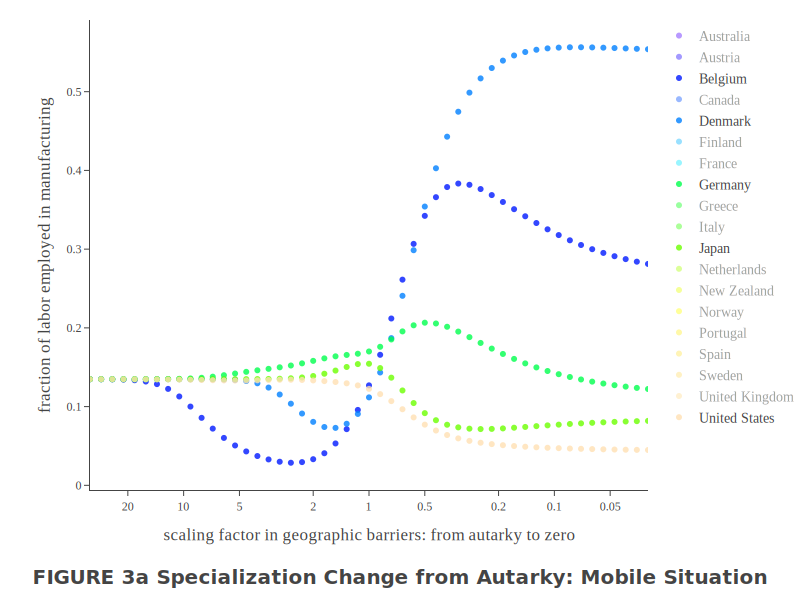
\includegraphics[width=1\linewidth]{img/Figure3} \end{center}

现存的地理障碍处在一种中间状态,地理因素和技术因素共同决定着贸易模式(国际分工)。地理障碍从目前水平下降将使技术因素变得更为重要,从而削弱大国的优势。

\hypertarget{ux5916ux56fdux6280ux672fux7684ux6ea2ux51faux6548ux5e94}{%
\subsection{外国技术的溢出效应}\label{ux5916ux56fdux6280ux672fux7684ux6ea2ux51faux6548ux5e94}}

在现有的地理障碍水平下,一国的技术进步可以通过贸易使全世界的福利改善,这个改善的国别分布是什么?我们先后令美国和德国的技术提高 20\%,来观察标准化的各国福利变化幅度(各国福利变化幅度除以技术进步国的福利变化幅度)。Table 11 显示了反事实模拟的结果。

\begin{center}\includegraphics[width=1\linewidth]{img/Table11} \end{center}

当劳动力可跨部门流动时,收入外生,福利只与价格有关。因为各国都享受到了价格更低的制造业产品,故各国福利普遍改善。

当劳动力不可跨部门流动时,他国福利同时还受到负收入效应的影响(因为制造业工资下降)。若一国不能降低其制造业就业规模,则该国总体福利常常会下降------日本和德国是典型。

离技术进步的国家越近和规模越小的国家,其福利改善的幅度越大。日本距离技术进步国既远,本身规模又大,从美国或德国的技术进步中得到的好处是最少的。

综上,充分享受他国技术进步的溢出效应需要两个条件:(1)距离技术进步源头足够近;(2)规模足够小,能够将更多劳动力向非制造业转移。

\hypertarget{ux524aux51cfux5173ux7a0e}{%
\subsection{削减关税}\label{ux524aux51cfux5173ux7a0e}}

我们的框架很容易结合关税收益。设进口国 \(n\) 在 \(i\)
国商品到岸价格的基础上征收从价税,税率为
\(t_{ni}\)。于是地理障碍可以拆分成自然地理障碍和关税两部分:\(d_{n i}=\left(1+t_{n i}\right) d_{n i}^{*}\)。关税收益为:

\[
T R_{n}=\sum_{i \neq n} \frac{t_{n i}}{1+t_{n i}} X_{n i}
\]

以所有国家对所有进口商品征收统一的 5\% 关税为 baseline,进行三种情境的反事实模拟:

\begin{enumerate}
\def\labelenumi{\arabic{enumi}.}
\item
  所有国家移除关税。劳动力可以跨部门流动时,所有国家的福利增加,且大于劳动力不可流动的情境。
\item
  美国单边移除关税。其他国家都有正的福利效应,而美国福利降低,其中加拿大的福利正效应最大。在劳动力流动情境下,其他所有国家的福利收益等于或大于美国的福利损失。这一结论说明了多边协调自由贸易的重要性(打破囚徒困境)。
\item
  欧洲共同体(EC)内部互相移除关税。Table 12
  表明,福利分配与劳动力是否可以跨部门流动密切相关。如第二列显示的,在劳动力不可流动时,主要的受害者是距离
  EC 比较近的非 EC
  成员国,它们的制造业工资下降了。在劳动力可以流动时,第一列显示,受害者是北方的
  EC 国家(比利时、荷兰、丹麦、德国、英国)。这种情境下,非 EC
  成员国可以通过将劳动力转移到非制造业来规避制造业工资的下降。北方 EC
  国家将进口来源从非成员国转向南方 EC
  国家。第三、四列表明,市场一体化使得成员国之间的贸易大量增加。而且在劳动力流动情形下,因投入品价格下降获得了一定的成本优势,EC
  国家对非 EC 国家的出口通常也扩大了。
\end{enumerate}

\begin{center}\includegraphics[width=1\linewidth]{img/Table12} \end{center}

\hypertarget{ux7ed3ux8bba}{%
\section{结论}\label{ux7ed3ux8bba}}

比较优势可以通过贸易创造潜在收益。然而,这些潜在收益的实现会受到地理障碍的削弱。我们的李嘉图模型可以非常简洁地捕捉这两种力量。该模型将双边贸易与技术和地理参数联系起来,我们使用了双边贸易流量、价格和地理数据(体现贸易障碍的各种代理变量)估计模型中的参数。

尽管引力模型的文献已经认识到了地理障碍在减少贸易量中的重要性,但\textbf{国际贸易的经典模型通常忽略了这些障碍}。例外情况是,阿明顿假设或垄断竞争模型,这些设定通过产品差异化预先决定了专业化模式。相反,我们的框架允许地理障碍和技术共同决定专业化模式。它还将贸易流量与(由地理壁垒产生的)各国价格水平对一价定律的偏离联系了起来。

  \bibliography{mybib.bib}

\end{document}
